\documentclass{beamer}

\usepackage{fancyvrb}
\usepackage{color, colortbl}
\usepackage{listings}
\usepackage{url}
\usepackage{array}
\usepackage{calc}
\usepackage{ctable}
\usepackage{amsmath}
\usepackage{cite}
\usepackage{graphicx}
\usepackage{listings}
\usepackage{xspace}
\usepackage{hyperref}
\usepackage{subfigure}
\usepackage{multicol}
\definecolor{lightgray}{rgb}{0.9,0.9,0.9}



\lstset{ %
language=C++,                % choose the language of the code
basicstyle=\tiny,       % the size of the fonts that are used for the code
%numbers=left,                   % where to put the line-numbers
numbers=none,                   % where to put the line-numbers
numberstyle=\scriptsize,      % the size of the fonts that are used for the line-numbers
stepnumber=1,                   % the step between two line-numbers. If it's 1 each line will be numbered
numbersep=15pt,                  % how far the line-numbers are from the code
backgroundcolor=\color{lightgray},  % choose the background color. You must add \usepackage{color}
%backgroundcolor=none,  % choose the background color. You must add \usepackage{color}
showspaces=false,               % show spaces adding particular underscores
showstringspaces=false,         % underline spaces within strings
showtabs=false,                 % show tabs within strings adding particular underscores
frame=single,	                % adds a frame around the code
%frame=none,	                % adds a frame around the code
tabsize=2,	                % sets default tabsize to 2 spaces
%captionpos=b,                   % sets the caption-position to bottom
captionpos=n,
%basicstyle=\small,
%basicstyle=\small\sffamily,
basicstyle=\sffamily\small,
%basicstyle=\ttfamily\small,
breaklines=true,                % sets automatic line breaking
breakatwhitespace=false,        % sets if automatic breaks should only happen at whitespace
columns=fullflexible,
title=\lstname,                 % show the filename of files included with \lstinputlisting; also try caption instead of title
escapeinside={\%*}{*)},          % if you want to add a comment within your code
morekeywords={chare,mainchare,module,mainmodule,entry,readonly,array,serial,for,when,if,then,else,overlap,while,forall,threaded,sync,message,group,nodegroup},
aboveskip=2pt,
belowskip=2pt,
lineskip=0pt,
xleftmargin=1em,
xrightmargin=1em,
%xleftmargin=10pt
abovecaptionskip=0pt,
belowcaptionskip=0pt,
}

\hypersetup{
    colorlinks,%
    citecolor=black,%
    filecolor=black,%
    linkcolor=black,%
    urlcolor=magenta
}


\newcommand{\charm}{Charm++}
\newcommand{\code}[1]{\colorbox{lightgray}{\texttt{#1}}}
\newcommand{\transition}[1]{\begin{frame}[plain]\begin{center}\LARGE #1\end{center}\end{frame}}
\newcommand{\comment}[1]{ }
\newcommand{\eat}[1]{ }

\DefineVerbatimEnvironment{codeverb}{Verbatim}{fontsize=\small}

\let \isForClass 1
\if \isForClass 1
  \newcommand{\removeForClass}[2]{#2}
  \else
  \newcommand{\removeForClass}[2]{#1}
\fi


\usefonttheme{professionalfonts}

\usetheme{Boadilla}
\usecolortheme{beaver}

\AtBeginSection[]{
  \frame<beamer>{
  \frametitle{Outline}
  \tableofcontents[currentsection]
 }
}

\title[Parallelism with Charm++]{Parallel Programming with \charm}
\institute[PPL, UIUC]{
\includegraphics[scale=0.8]{../figures/illinois_logo-crop.pdf}\\Parallel Programming Lab\\ University of Illinois}
\author[Phil and Ram]{Laxmikant Kal\'e, Phil Miller, Ramprasad Venkataraman}
\date{May 14, 2012}

\begin{document}

\frame{\titlepage}

\section{Why Parallelism}
\section{Motivating Challenges}
\section{\charm}
\begin{frame}[t]
\frametitle{\charm}
\framesubtitle{}
	\begin{block}{Parallel ...}
		\begin{itemize}[<+->]
		\item \alert<4->{... programming model}
		\item ... programming framework
		\item ... runtime system
	\end{itemize}
	\end{block}
    \begin{itemize}[<+->]
        \item General-purpose
        \item Macro Dataflow
        \item Unified data and task parallelism
        \item Unified handling of shared and distributed memory
        \item Parallel algorithm independent of available processors
        \item Seamless parallel composability of modular components
    \end{itemize}
\end{frame}


\begin{frame}[t]
\frametitle{\charm}
\framesubtitle{}
	\begin{block}{Parallel ...}
		\begin{itemize}
		\item ... programming model
		\item \alert{... programming framework}
		\item ... runtime system
	\end{itemize}
	\end{block}
    \begin{itemize}[<+->]
        \item Code generation, Base classes, utility functions and other API
        \item Multi-paradigm parallel code (procedural, object oriented, generic)
        \item Rich ecosystem of tools
        \item Separation of roles and concerns
        %\item Abstracts domain logic from parallel tuning
    \end{itemize}
\end{frame}


\begin{frame}[t]
\frametitle{\charm}
\framesubtitle{}
	\begin{block}{Parallel ...}
		\begin{itemize}
		\item ... programming model
		\item ... programming framework
		\item \alert{... runtime system}
	\end{itemize}
	\end{block}
    \begin{itemize}[<+->]
        \item Managed parallel execution
        %\item Shared-nothing by default, explicit sharing for optimization
        \item Measurement-based performance introspection
        \item Adaptive response for better performance
        \begin{itemize}
            \item Fault tolerance
            \item Dynamic load balancing
            \item Energy management
        \end{itemize}
    \end{itemize}
\end{frame}


\begin{frame}
\frametitle{\charm: Portability}
{\scriptsize
\onslide<1->{
\begin{block}{\small Environments}
    \begin{columns}
    \begin{column}{0.45\textwidth}
        \begin{itemize}
            \item Embedded ARM: CARMA dev boards, cell phones
            \item Commodity x86: servers, desktops, laptops, tablets
        \end{itemize}
    \end{column}
    \begin{column}{0.45\textwidth}
        \begin{itemize}
            \item Clusters: commodity, with a network
            \item Supercomputers: IBM Blue Gene and POWER, Cray
        \end{itemize}
    \end{column}
    \end{columns}
\end{block}
}
\only<1>{ 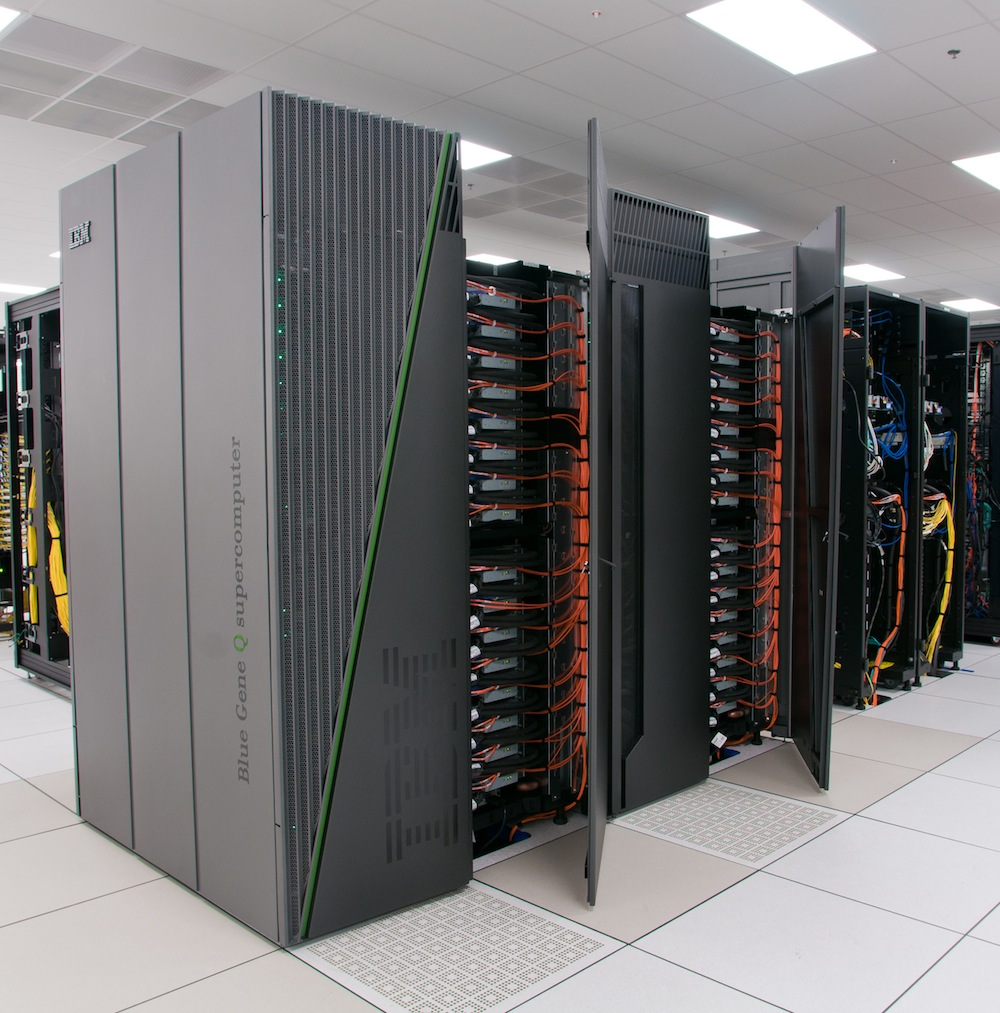
\includegraphics[width=0.48\textwidth]{../figures/mira.jpg} }
\only<1>{ 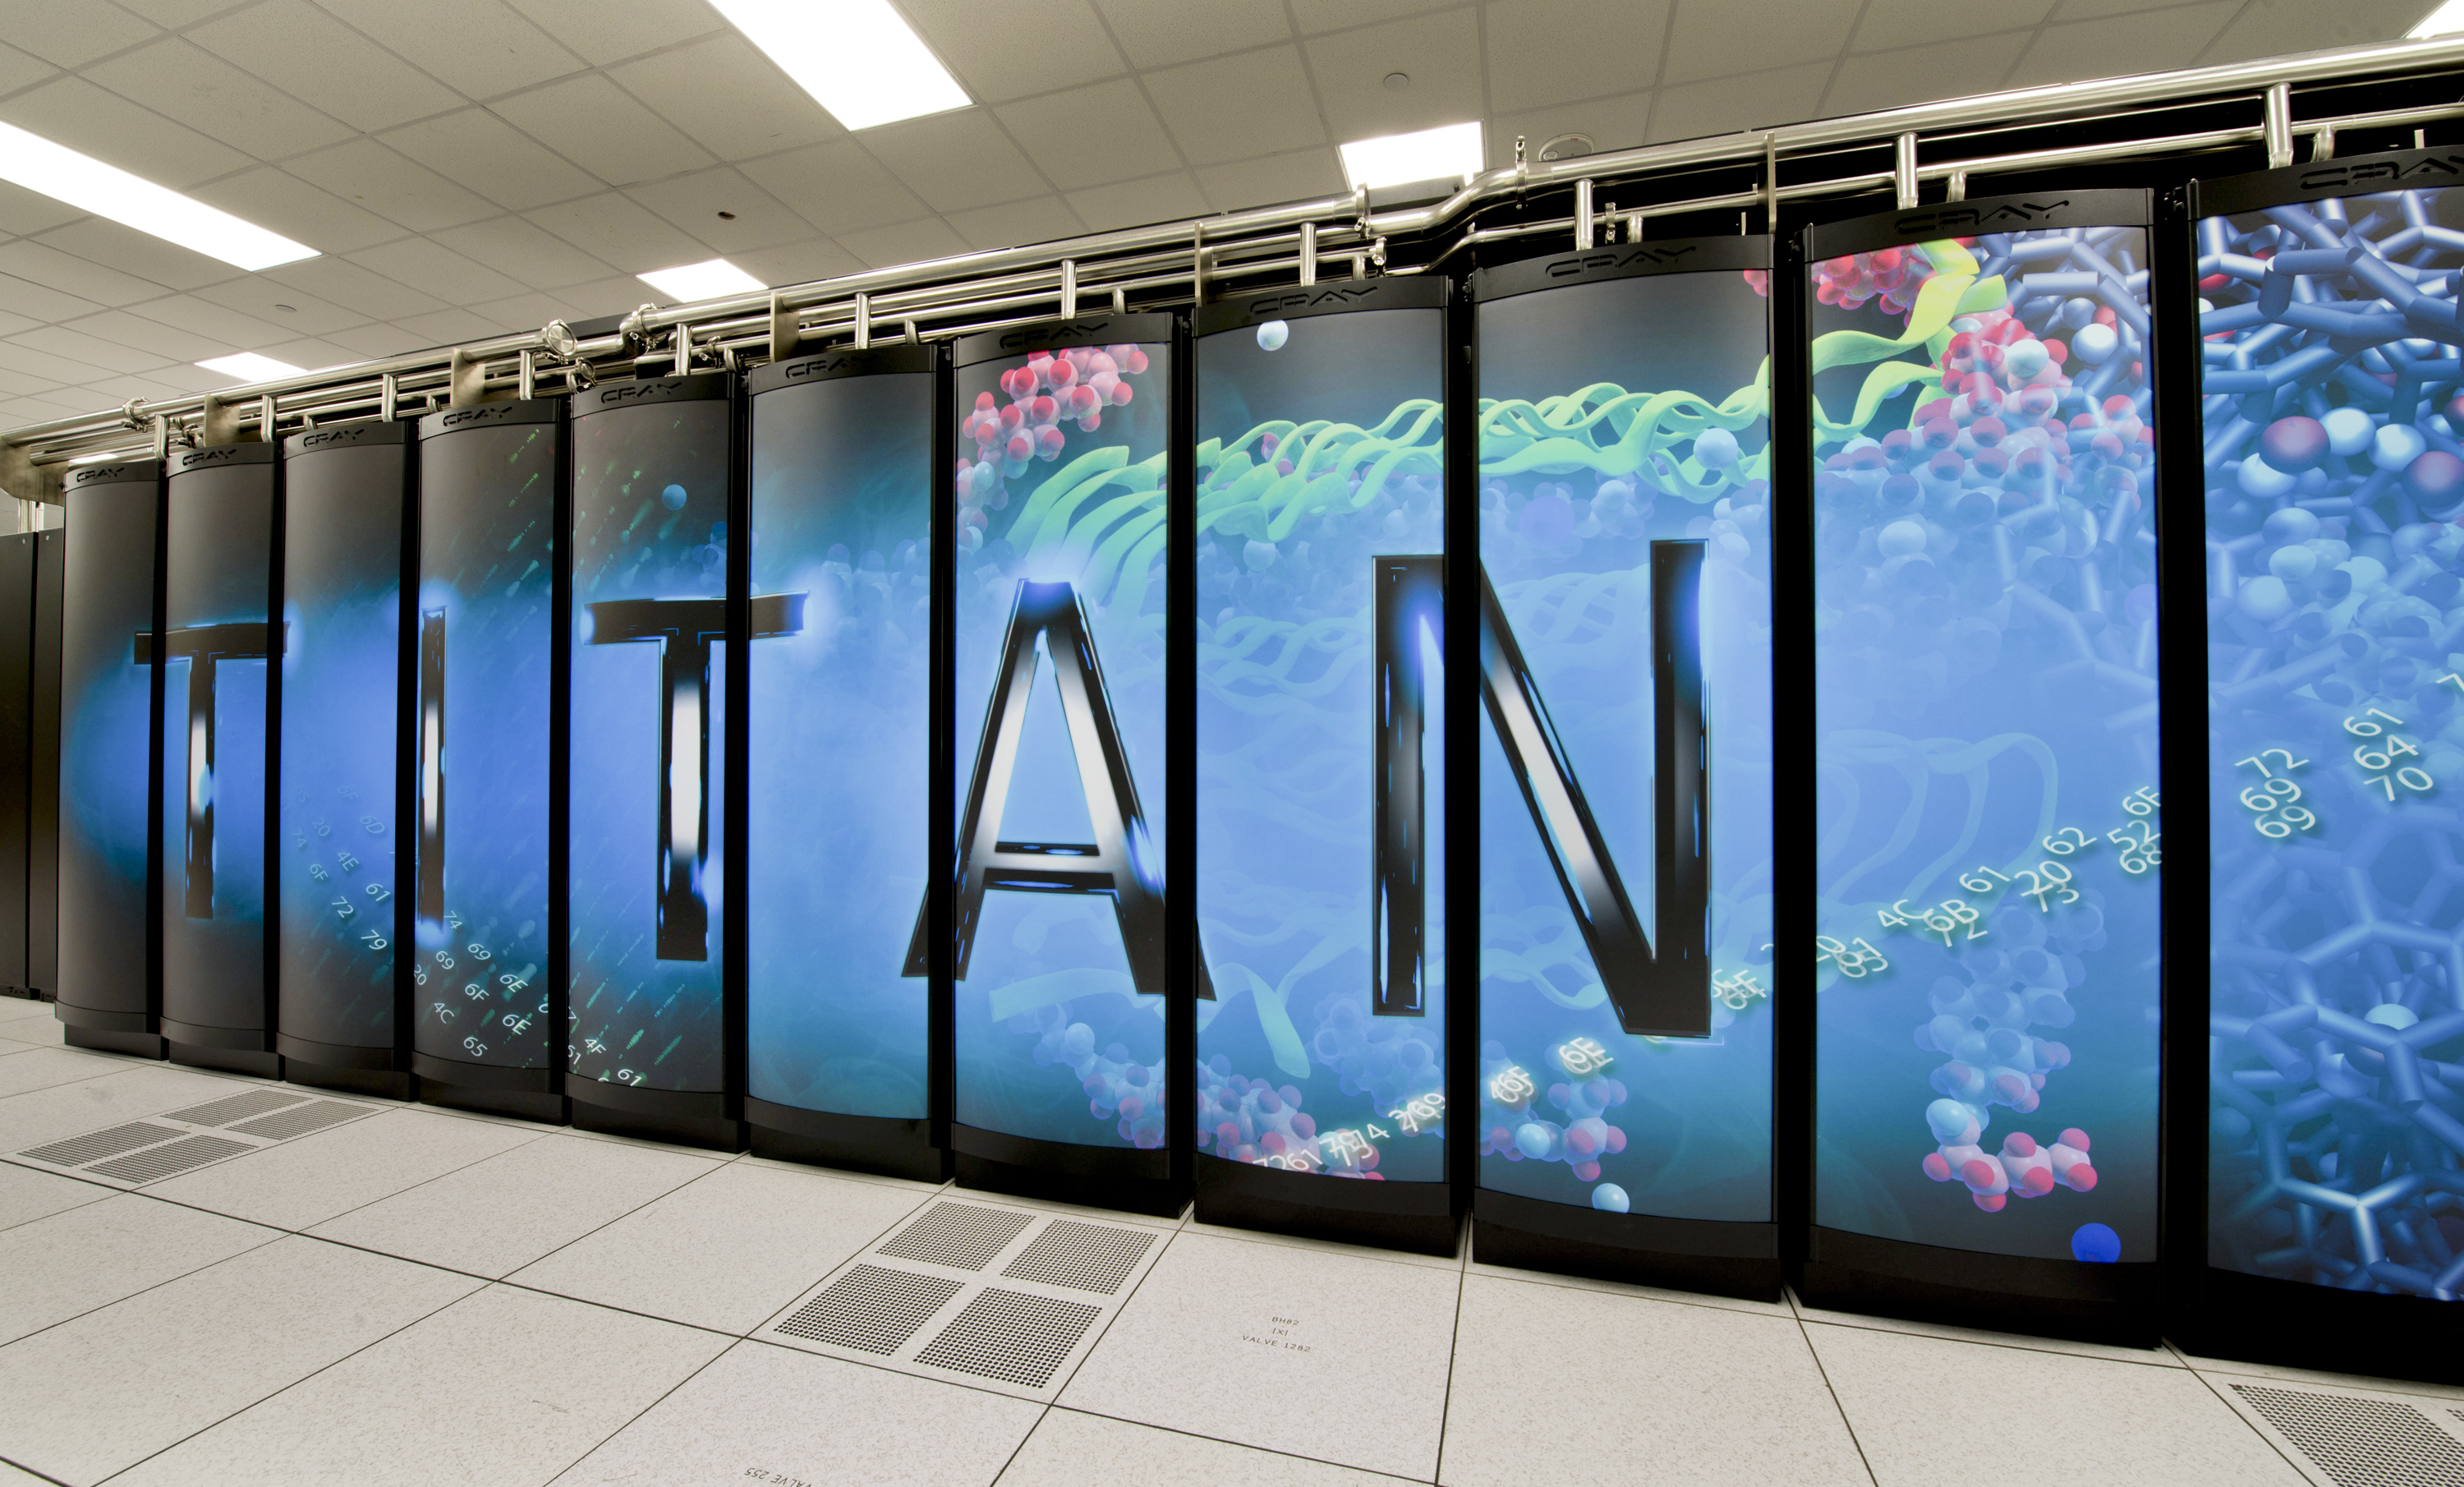
\includegraphics[width=0.48\textwidth]{../figures/titan.jpg} }
\onslide<2->{
\begin{block}{\small Operating Systems}
    \begin{columns}
    \begin{column}{0.45\textwidth}
        \begin{itemize}
            \item Linux
            \item Mac OS X
        \end{itemize}
    \end{column}
    \begin{column}{0.45\textwidth}
        \begin{itemize}
            \item Windows
            \item Proprietary Cray \& IBM
        \end{itemize}
    \end{column}
    \end{columns}
\end{block}
}
\only<3>{
\begin{block}{\small Network Interfaces}
    \begin{columns}
    \begin{column}{0.45\textwidth}
        \begin{itemize}
            \item TCP, UDP
            \item Shared memory
            \item MPI
        \end{itemize}
    \end{column}
    \begin{column}{0.45\textwidth}
        \begin{itemize}
            \item Infiniband Verbs
            \item IBM BlueGene P,Q (DCMF, PAMI)
            \item Cray Gemini and Aries (uGNI)
        \end{itemize}
    \end{column}
    \end{columns}
\end{block}
}
\onslide<4->{
\begin{block}{\small Compilers}
    \begin{columns}
    \begin{column}{0.45\textwidth}
        \begin{itemize}
            \item GCC
            \item Clang
            \item Microsoft VC++
            \item IBM XL
        \end{itemize}
    \end{column}
    \begin{column}{0.45\textwidth}
        \begin{itemize}
            \item Intel
            \item Portland Group (PGI)
            \item Cray
            \item Fujitsu
        \end{itemize}
    \end{column}
    \end{columns}
\end{block}
}
}
\end{frame}


\begin{frame}
\frametitle{\charm: Pedigree}
\begin{itemize}
\item 1987: Chare Kernel arose from parallel Prolog work
\item 1992: Initial C++-based Charm++
\item 1994-1996: NAMD developed
\item 1997: Application-facing abstractions reach near-current form
\item 1997: Adaptive MPI (AMPI) built atop Charm++
\item 2000-present: More applications developed, runtime facilities extended, scaling with new machines
\end{itemize}
\pause
\begin{block}{Award-winning}
Gordon Bell prize in 2002, HPC Challenge award in 2011, 2012 Sidney Fernbach prize for Kal\'e, several best papers
\end{block}
\end{frame}

\section{Expressing Parallel Algorithms}
\begin{frame}
  \frametitle{Express Parallel Algo independent of processors}
  \begin{figure}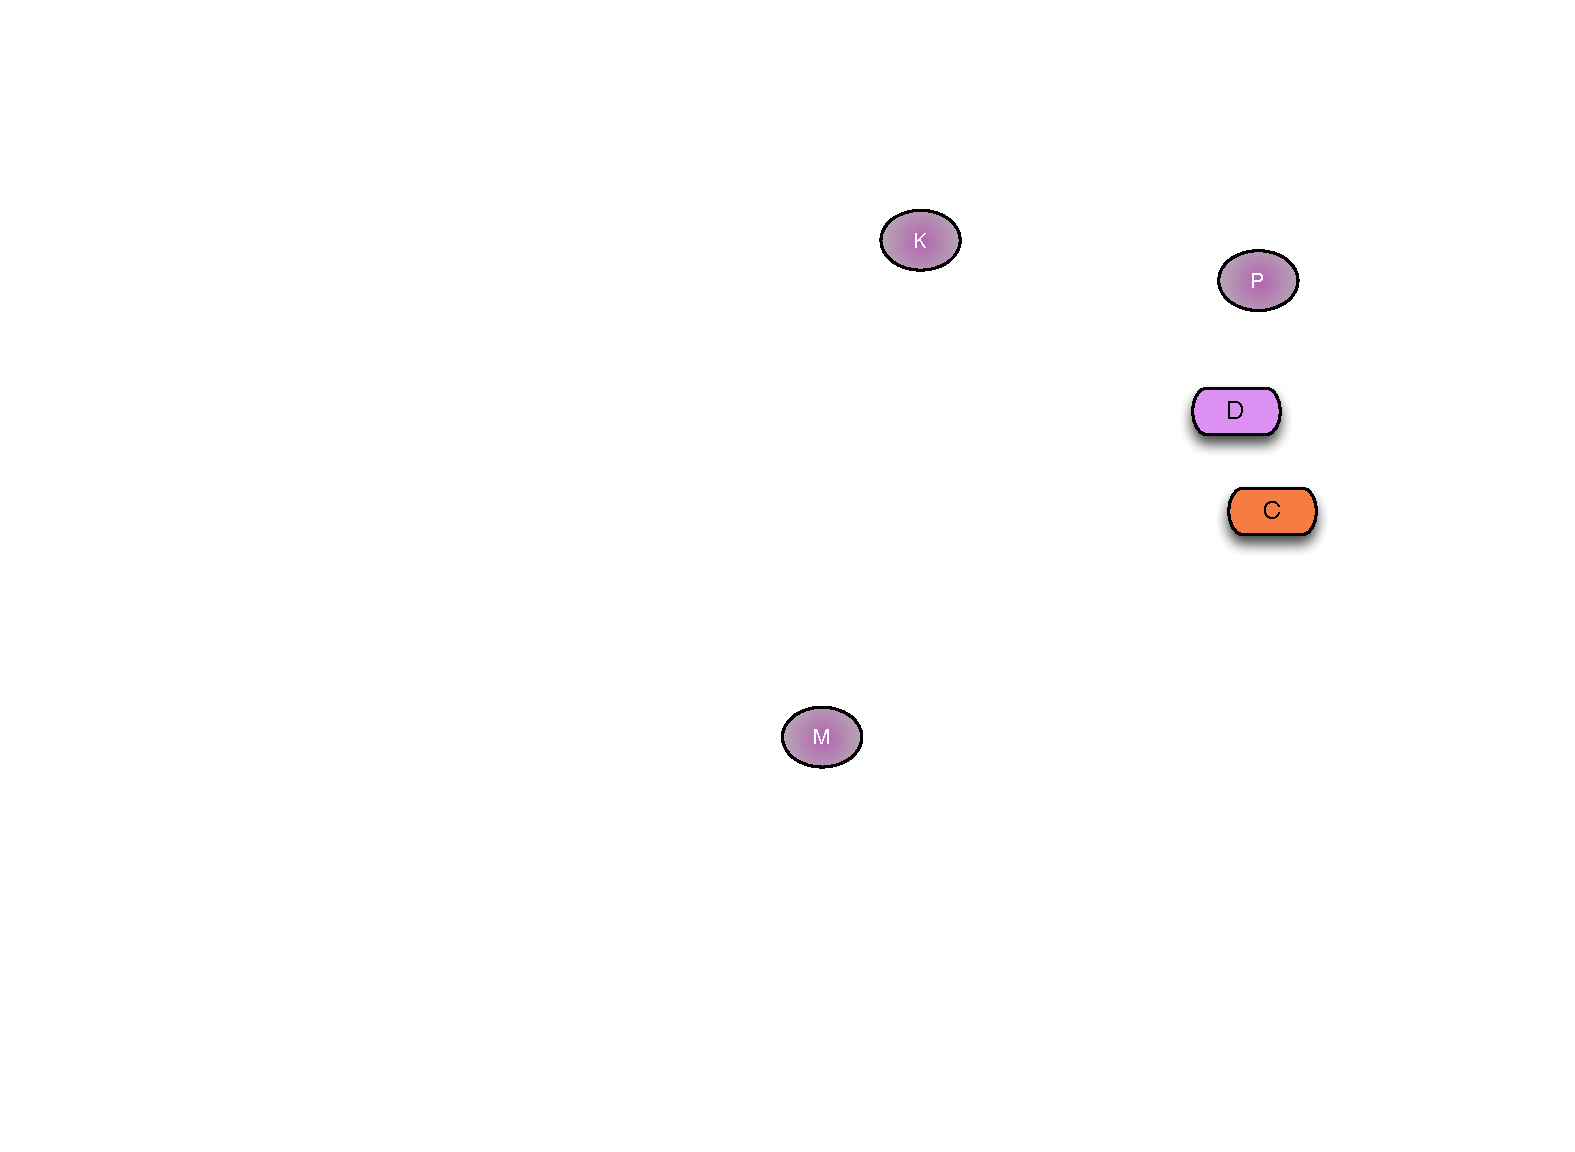
\includegraphics[width=0.9\textwidth]{../figures/progmodel/01-objects-for-algo.pdf}\end{figure}
\end{frame}


\begin{frame}
  \frametitle{Data parallelism: via an Object Collection}
  \begin{figure}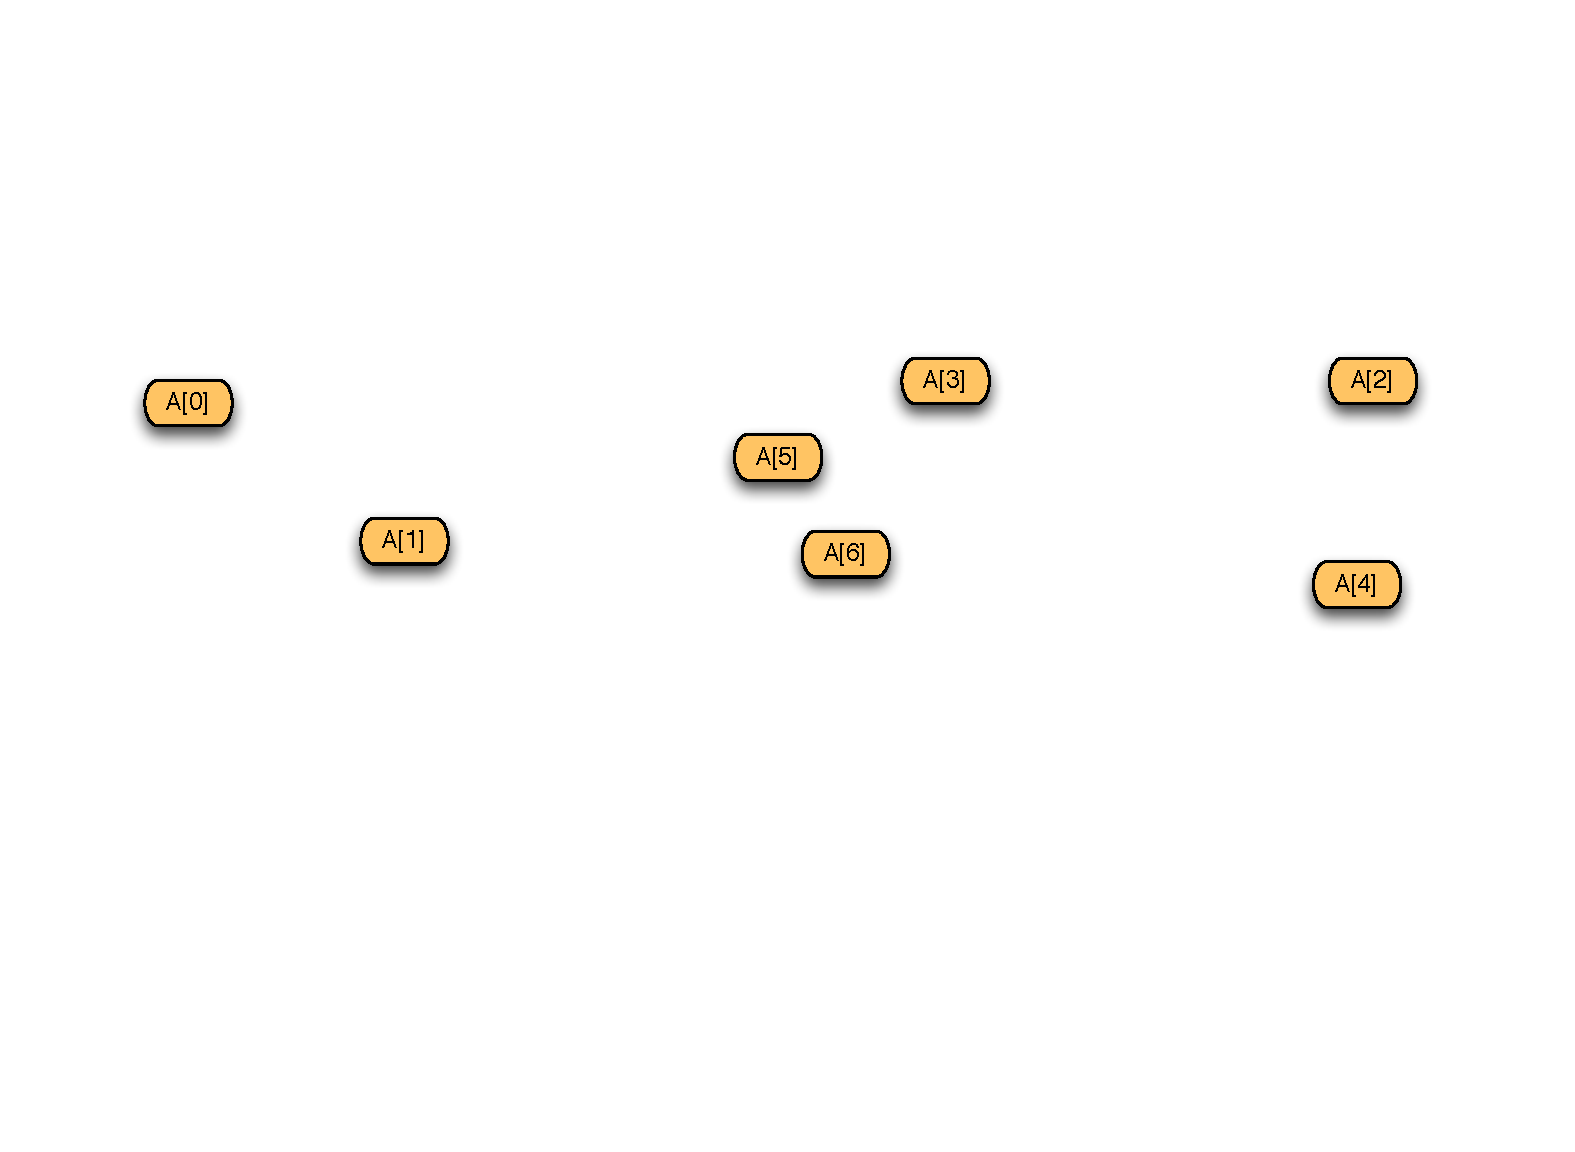
\includegraphics[width=0.9\textwidth]{../figures/progmodel/02-data-decomp-via-arrays.pdf}\end{figure}
\end{frame}


\begin{frame}
  \frametitle{Multiple data parallel collections}
say 2 matrices
  \begin{figure}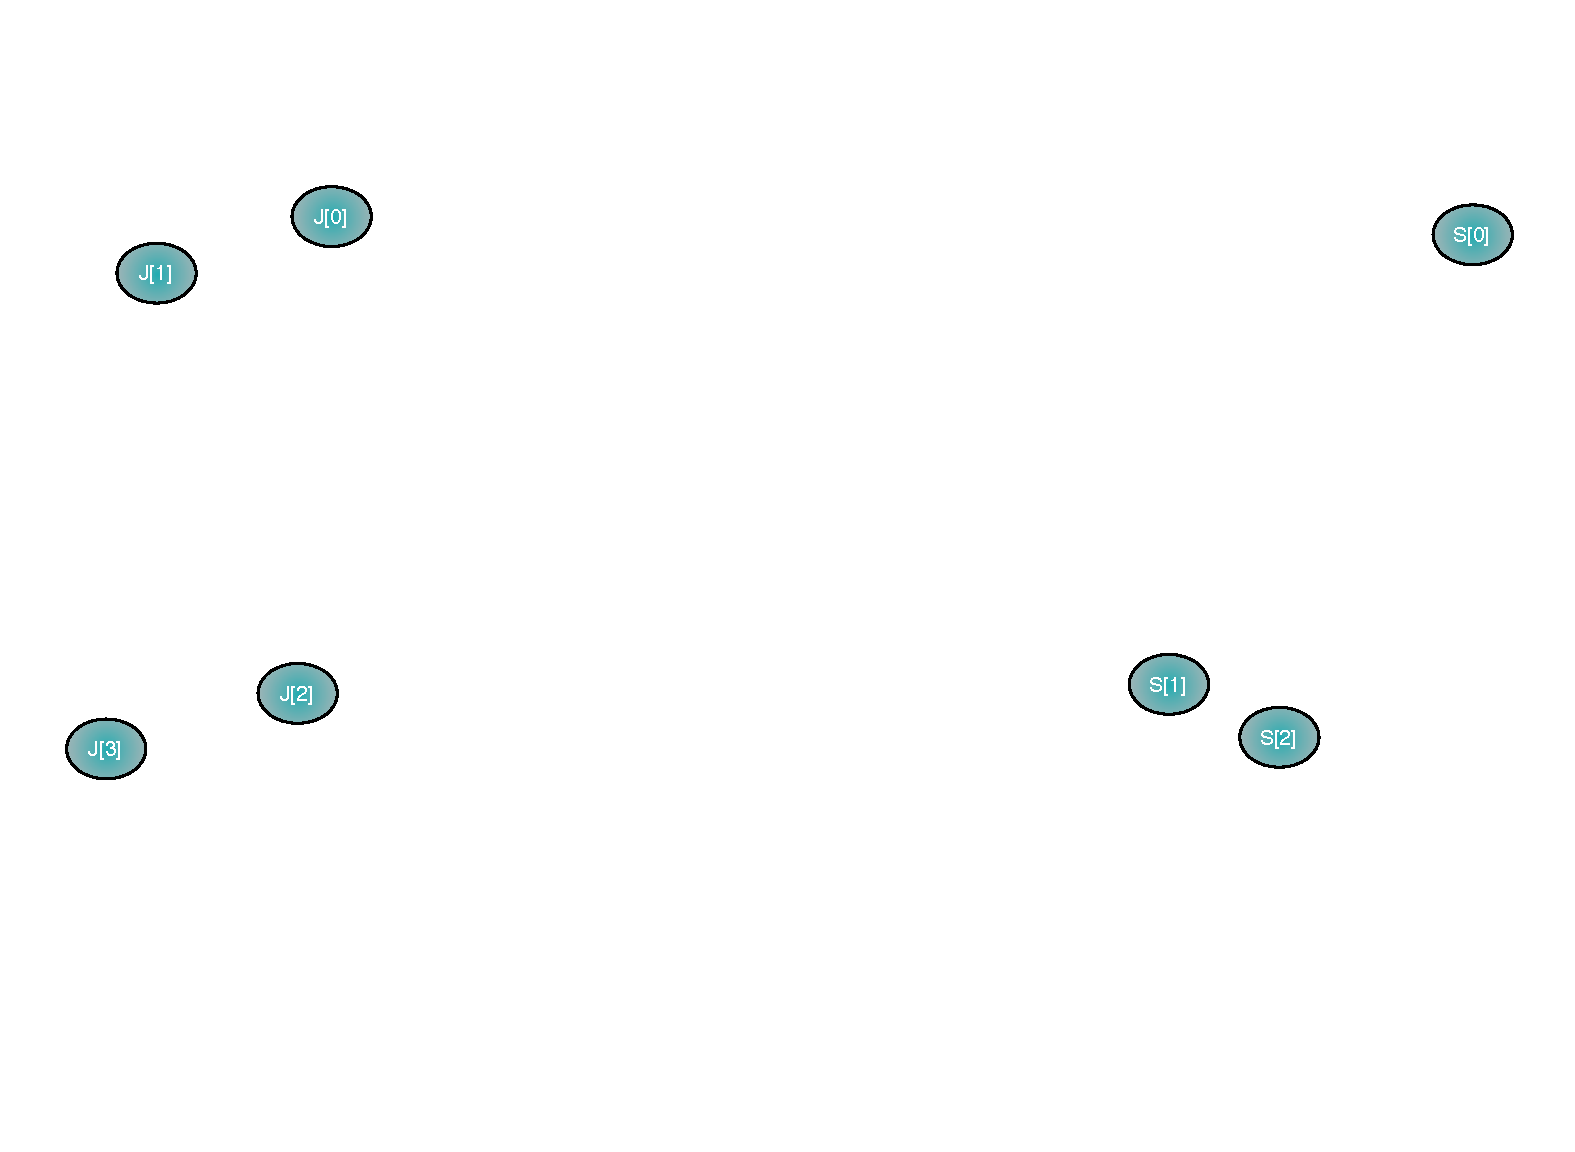
\includegraphics[width=0.9\textwidth]{../figures/progmodel/03-many-data-parallel-arrays.pdf}\end{figure}
\end{frame}


\begin{frame}
  \frametitle{Functional parallelism: via multiple classes}
  \begin{figure}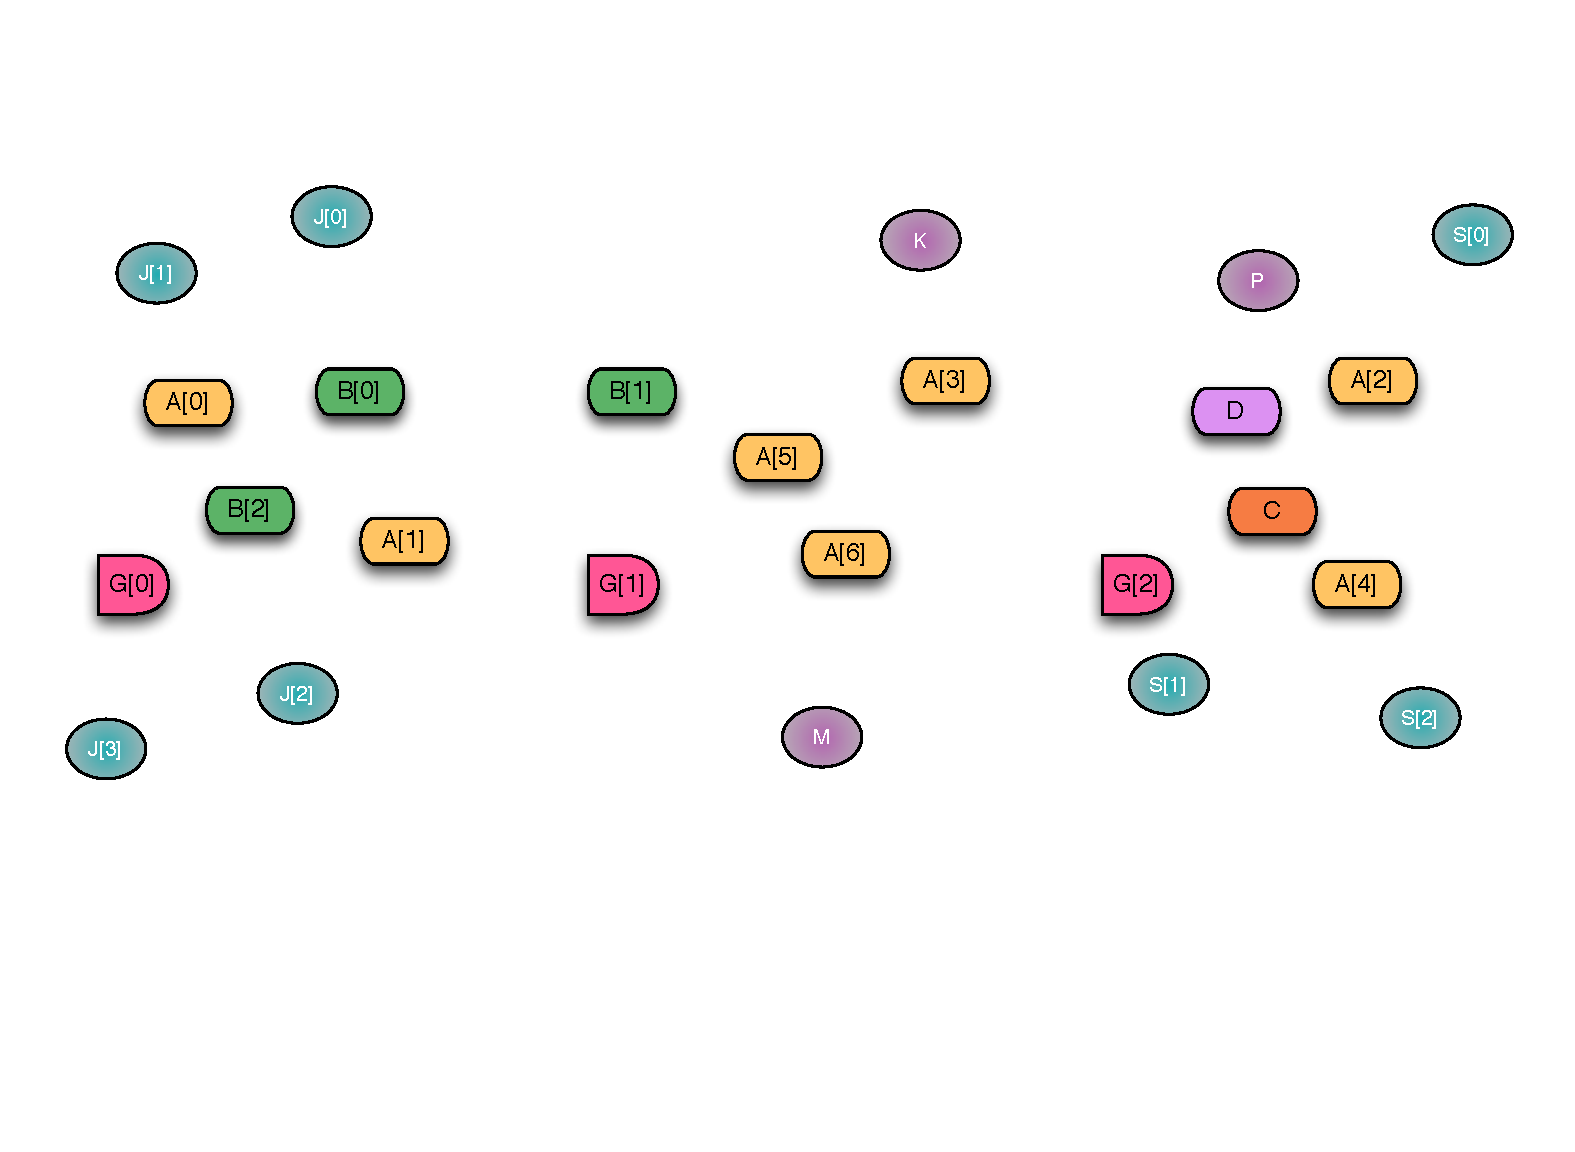
\includegraphics[width=0.9\textwidth]{../figures/progmodel/04-func-decomp-via-classes.pdf}\end{figure}
\end{frame}


\begin{frame}
  \frametitle{App logic: via classes and objects collections}
  \begin{figure}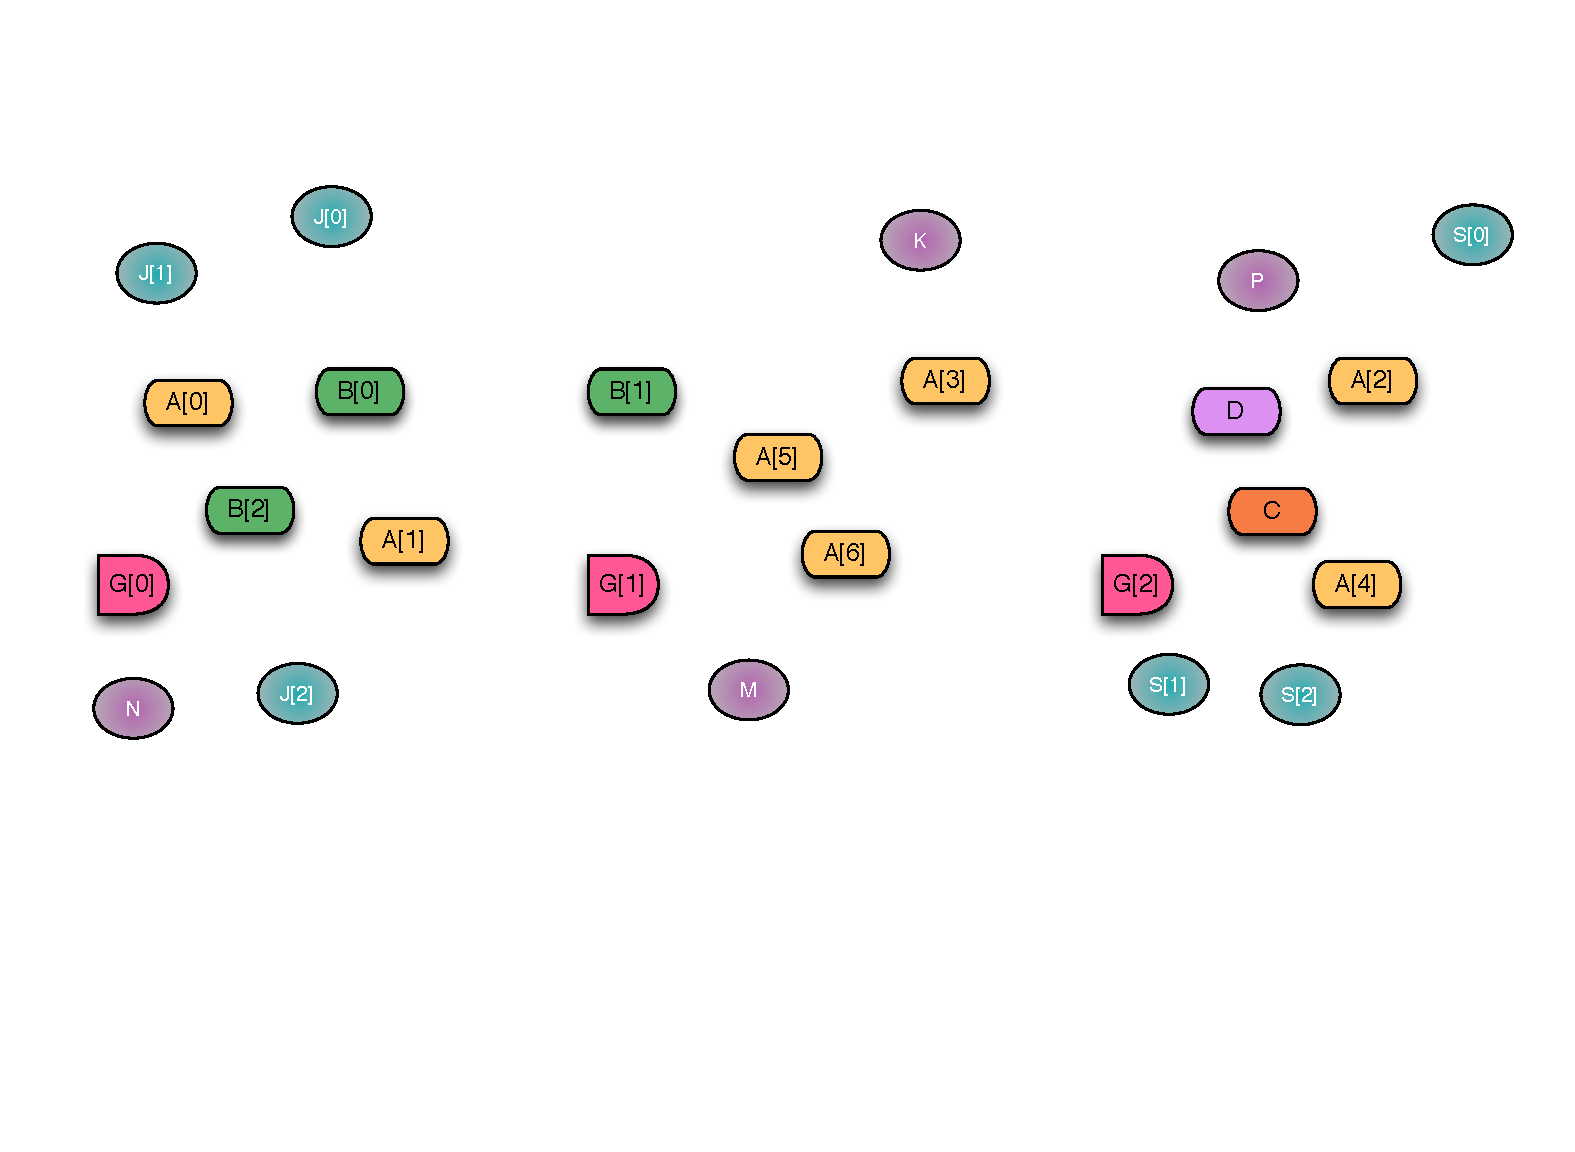
\includegraphics[width=0.9\textwidth]{../figures/progmodel/05-parallelism-via-obj-collections.pdf}\end{figure}
\end{frame}


\begin{frame}
  \frametitle{
    \only<1>{Parallelism requires distributing objects across processors}
    \only<2>{However, do not burden programmer with this view}
  }
  \begin{figure}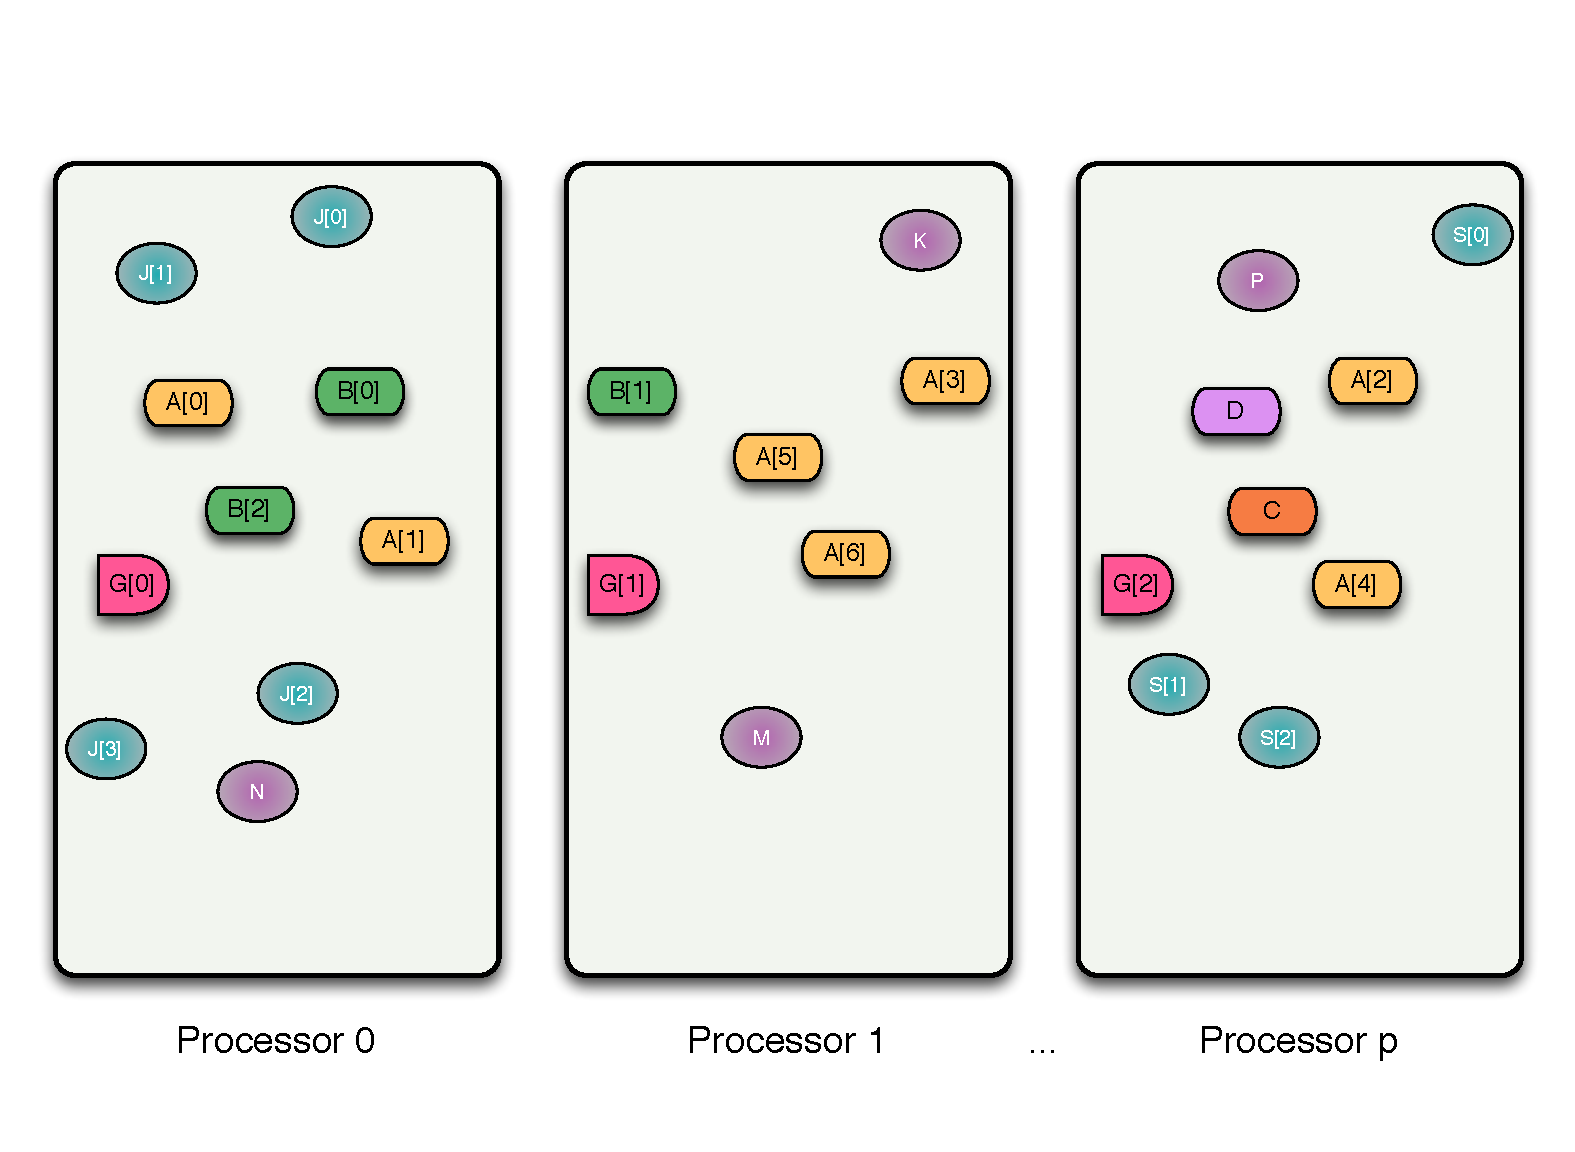
\includegraphics[width=0.9\textwidth]{../figures/progmodel/06-objects-sys-view.pdf}\end{figure}
\end{frame}


\begin{frame}
  \frametitle{
    \only<1>{Elevate some objects to global visibility}
    \only<3>{Globally visible objects = chares}
    \only<4>{Globally visible object collections = chare arrays}
  }
  \begin{figure}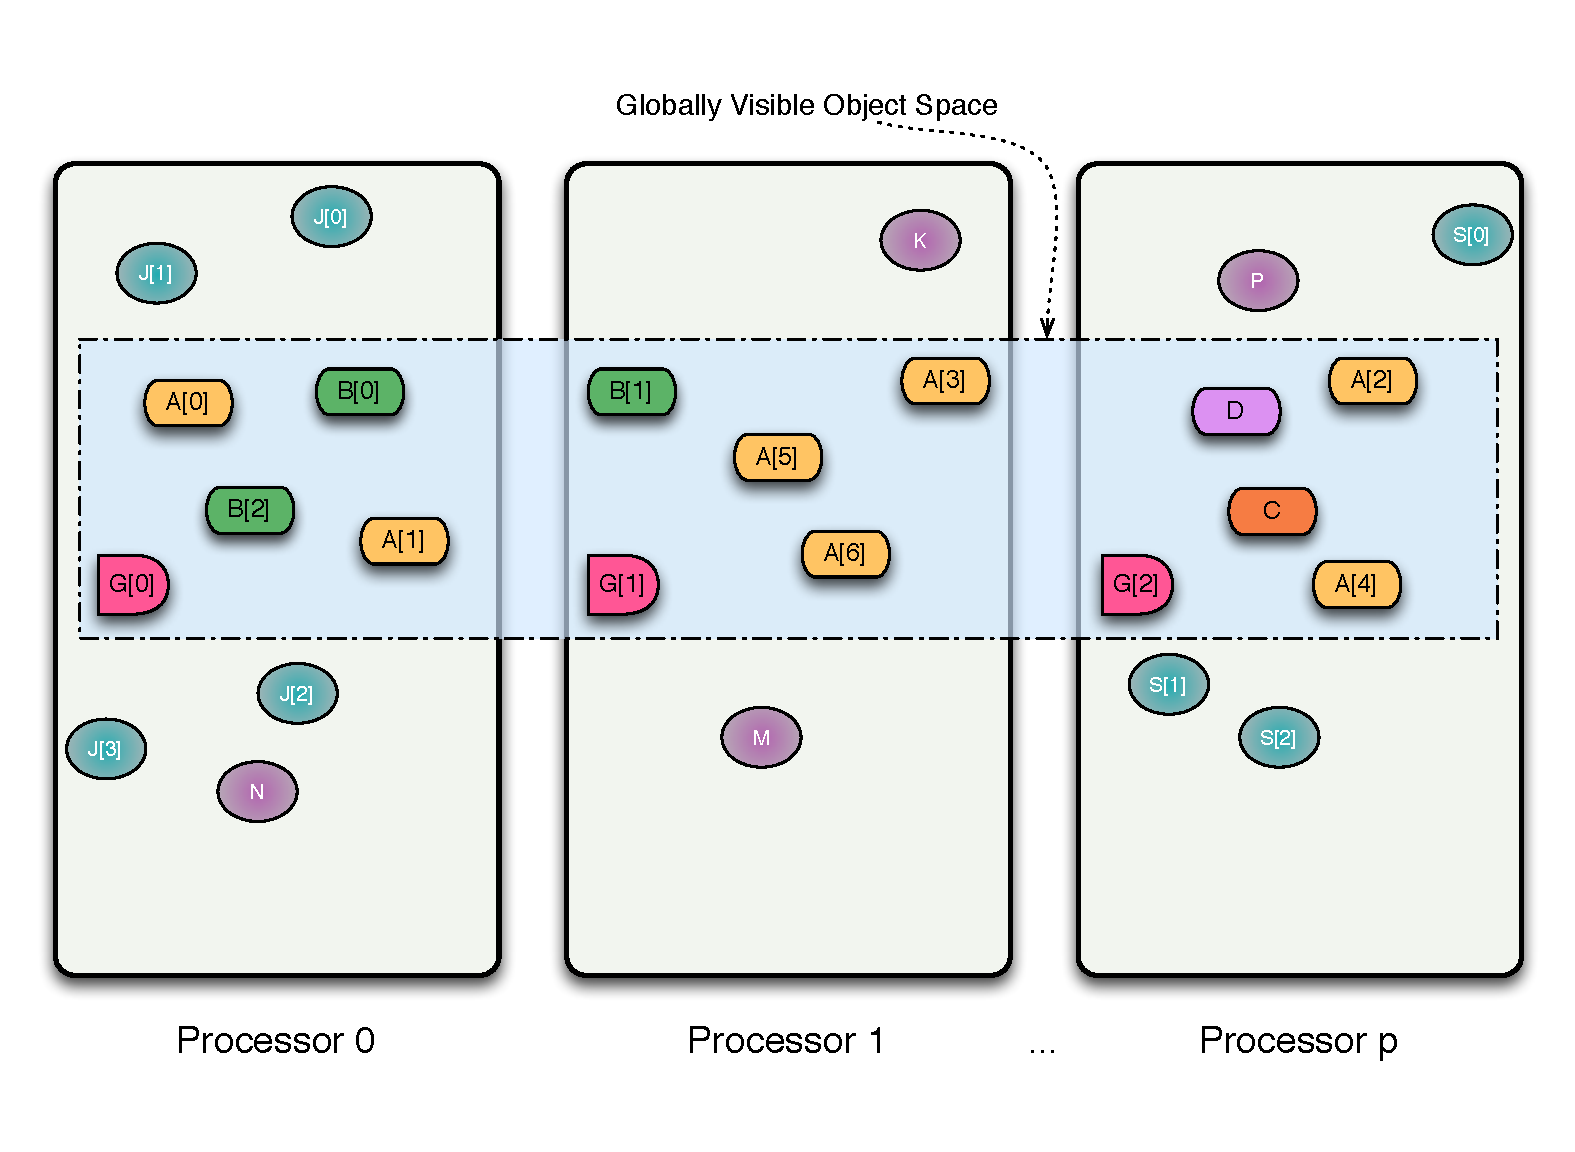
\includegraphics[width=0.9\textwidth]{../figures/progmodel/07-obj-programmer-view.pdf}\end{figure}
\end{frame}


\begin{frame}[fragile,t]
\frametitle{Annotating classes to enable global visibility}
\begin{columns}[t]
\begin{column}{0.4\textwidth}
\begin{block}{In \texttt{foo.ci}}
\begin{lstlisting}
module foo_module {
  array [2D] Foo {
    // . . .
  };
}
\end{lstlisting}
\end{block}
\end{column}
%\hspace{0.1\textwidth}
\begin{column}{0.5\textwidth}
\begin{block}{In \texttt{foo.h}}
\begin{lstlisting}
#include "foo_module.decl.h"

class Foo : public CBase_Foo {
  // . . . 
];
\end{lstlisting}
\end{block}
\begin{block}{In \texttt{foo.C}}
\begin{lstlisting}
#include "foo.h"

// . . . 

#include "foo_module.def.h"
\end{lstlisting}
\end{block}
\end{column}
\end{columns}
\end{frame}


\begin{frame}
\frametitle{Indexing into Object Collections}
    \begin{itemize}
       \item multidimensional, integer (1D .. 6D)
        \begin{itemize}
            \item Dense
            \item Sparse
        \end{itemize}
       \item anything hashable (strings, bitvectors)
       \item Static
       \item Dynamics (elements come and go)
    \end{itemize}
\end{frame}


\begin{frame}
\frametitle{Quantum Chemistry: OpenAtom}
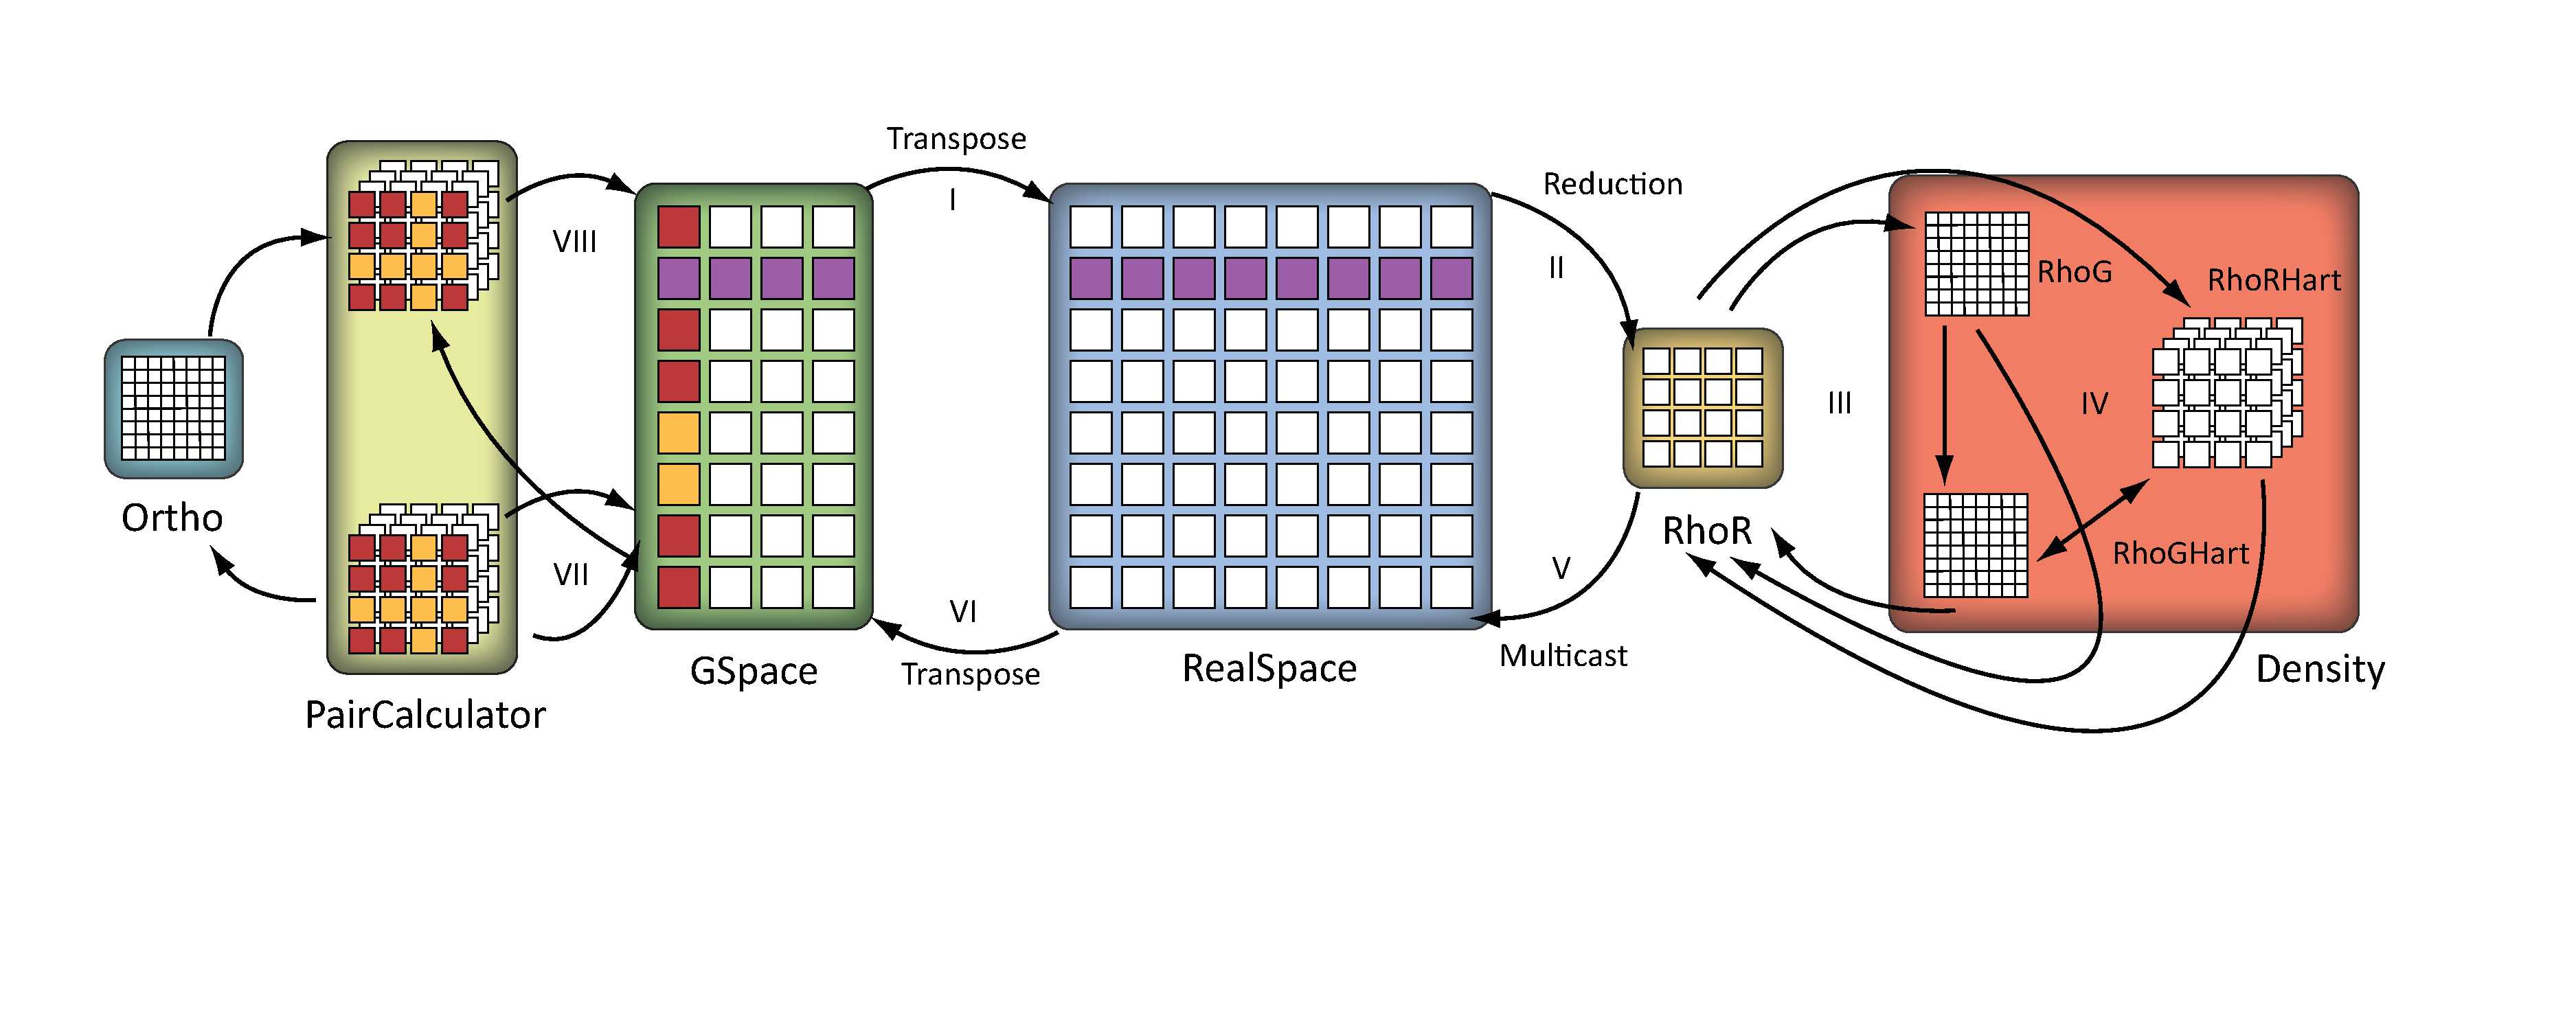
\includegraphics[width=\textwidth]{../figures/openatom/control-flow.pdf}
\end{frame}


\begin{frame}
\frametitle{Quantum Chemistry: OpenAtom}
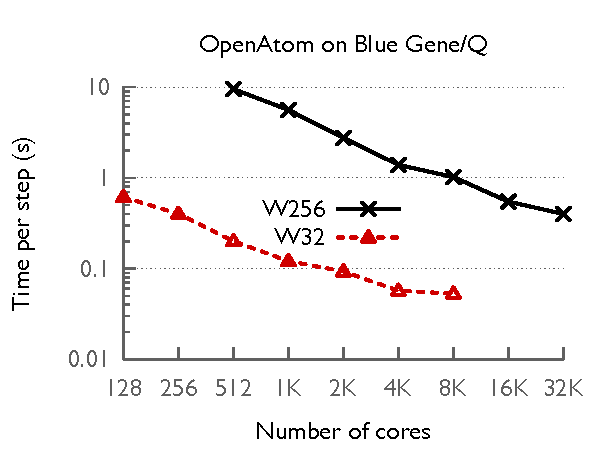
\includegraphics[width=\textwidth]{../figures/openatom/bgq.pdf}
\end{frame}



\section{Asynchronous Execution and Scheduling}
\begin{frame}
  \frametitle{Messages ...
    \only<1>{help objects communicate}
    \only<2>{express algorithmic dependencies}
    \only<3>{drive the parallel computation}
  }
  \begin{figure}
  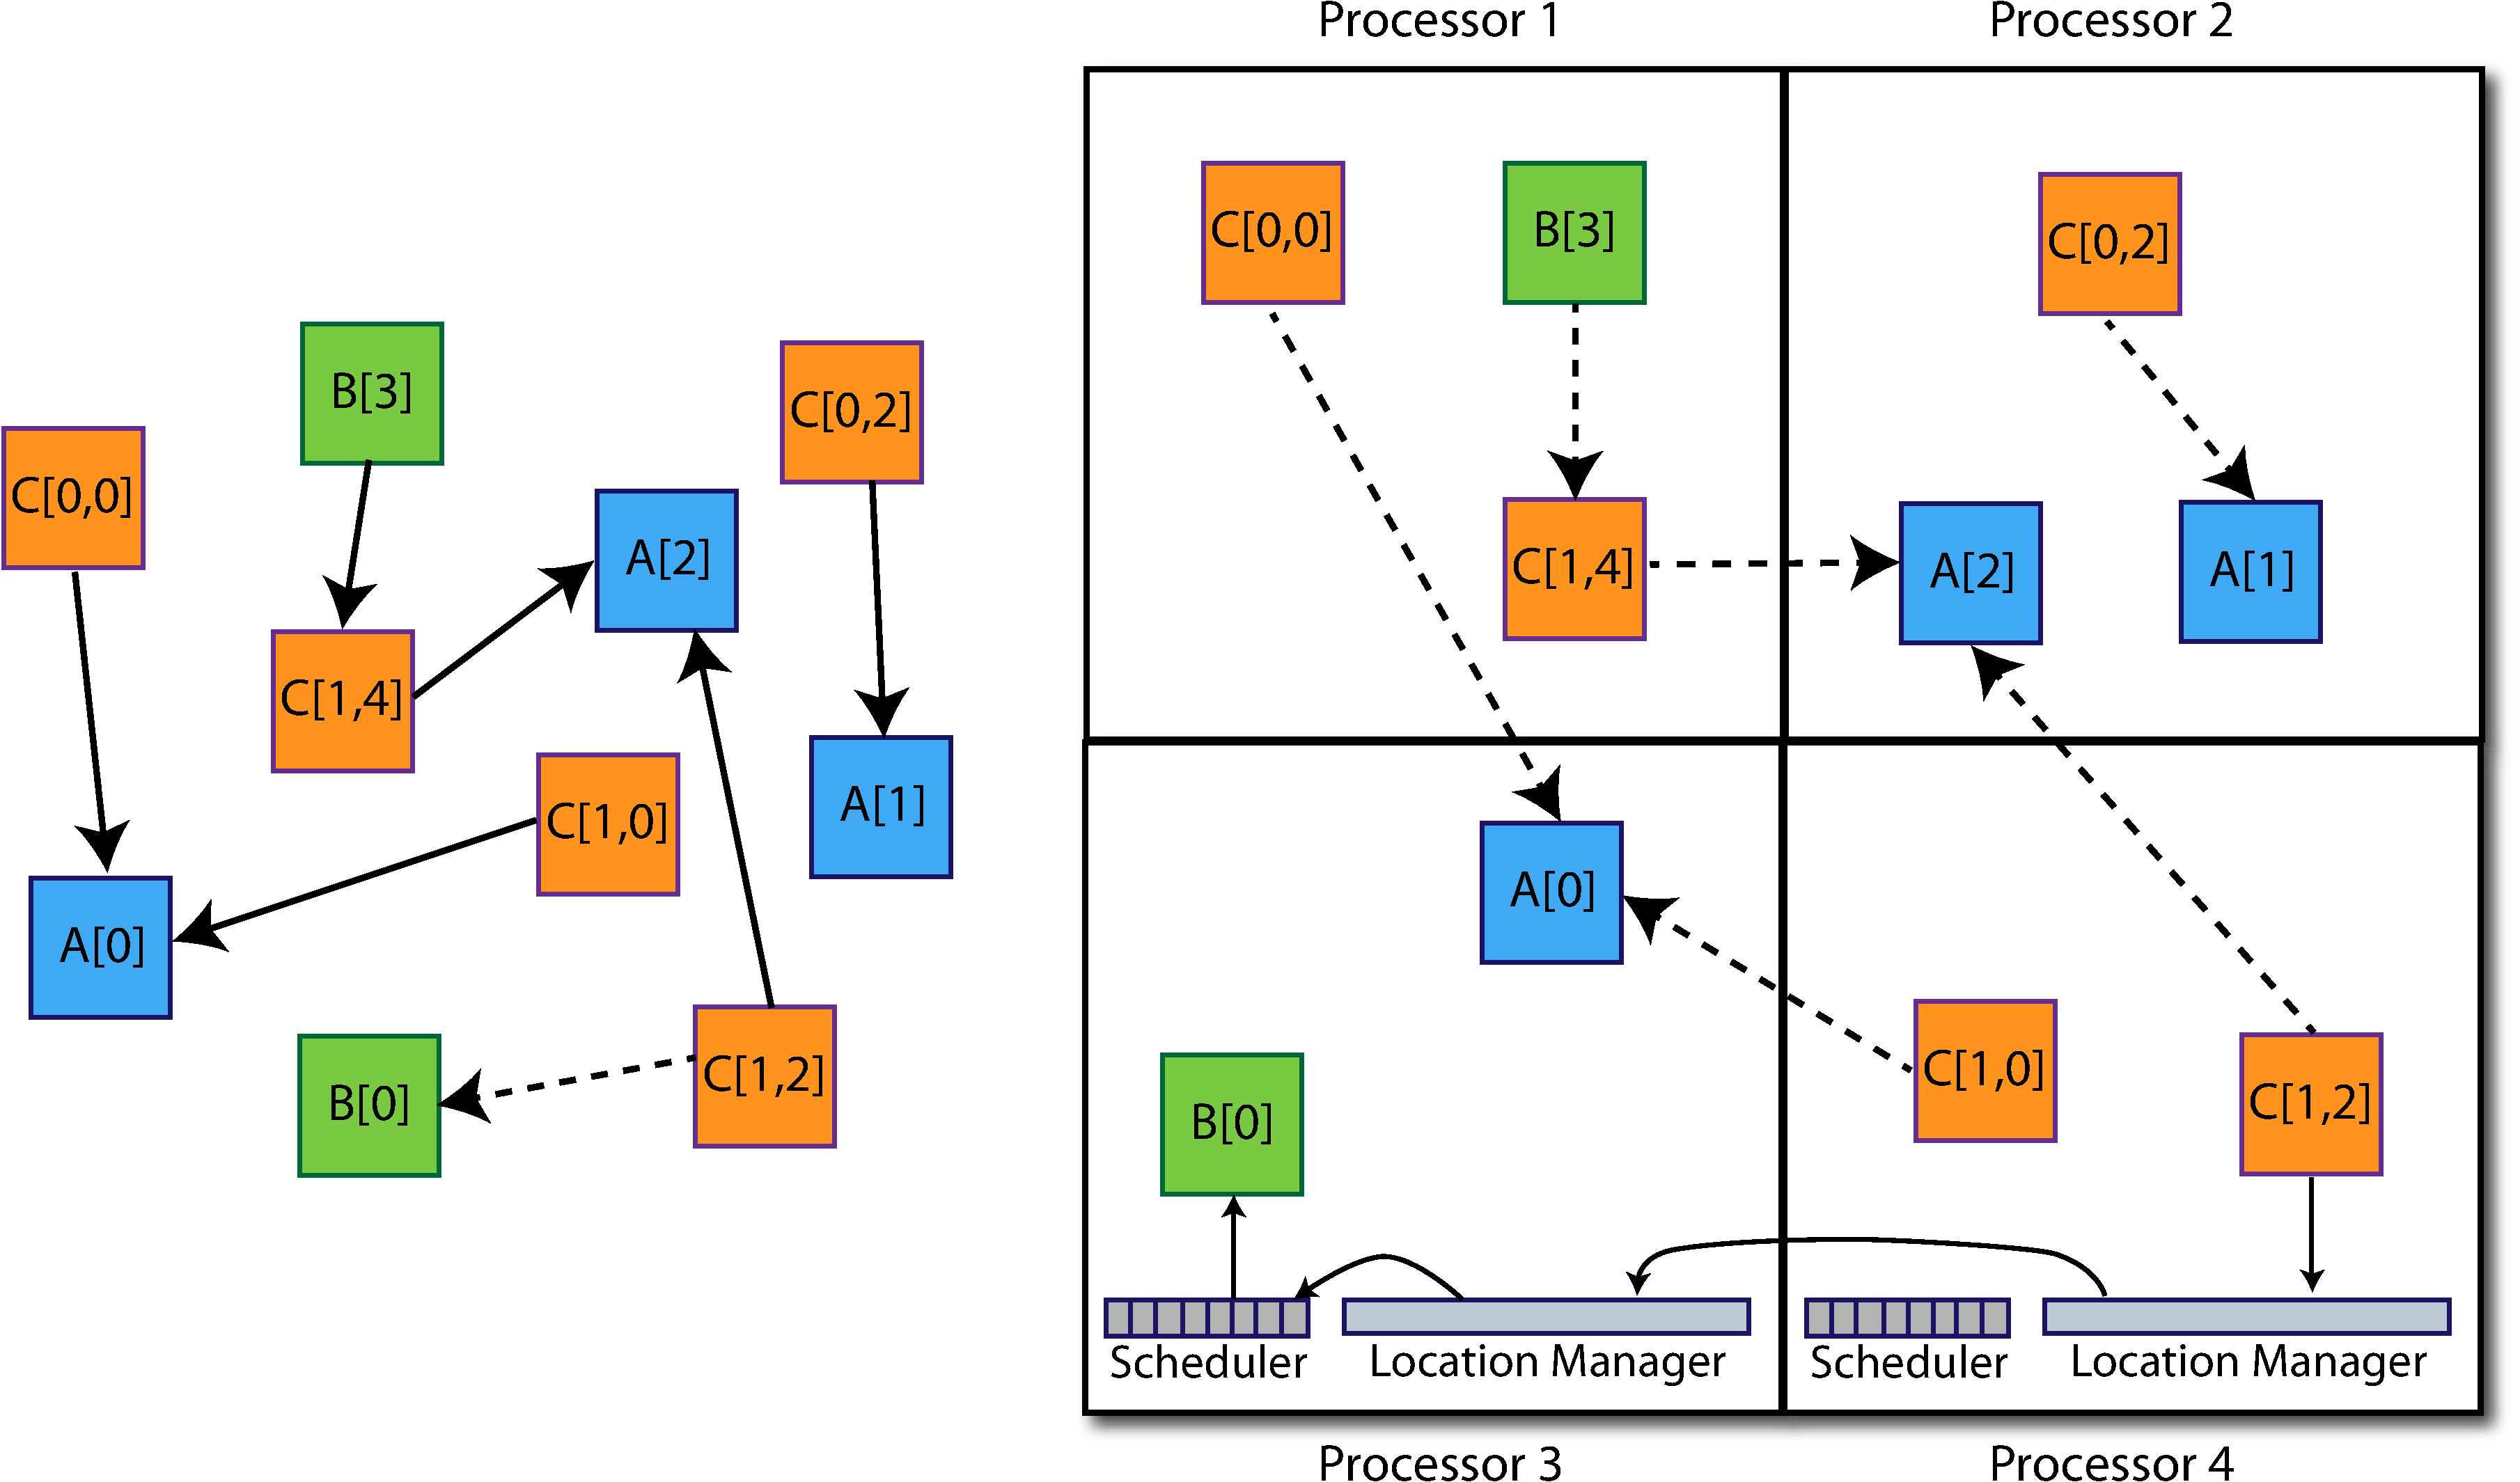
\includegraphics[trim=0in 0in 14in 2in, clip=true, height=0.85\textheight]{../figures/elements2.pdf}
  \end{figure}
\end{frame}

\begin{frame}
  \frametitle{Messages ...
    \only<1>{wait in queues}
    \only<2>{and are scheduled for execution}
  }
  \begin{center}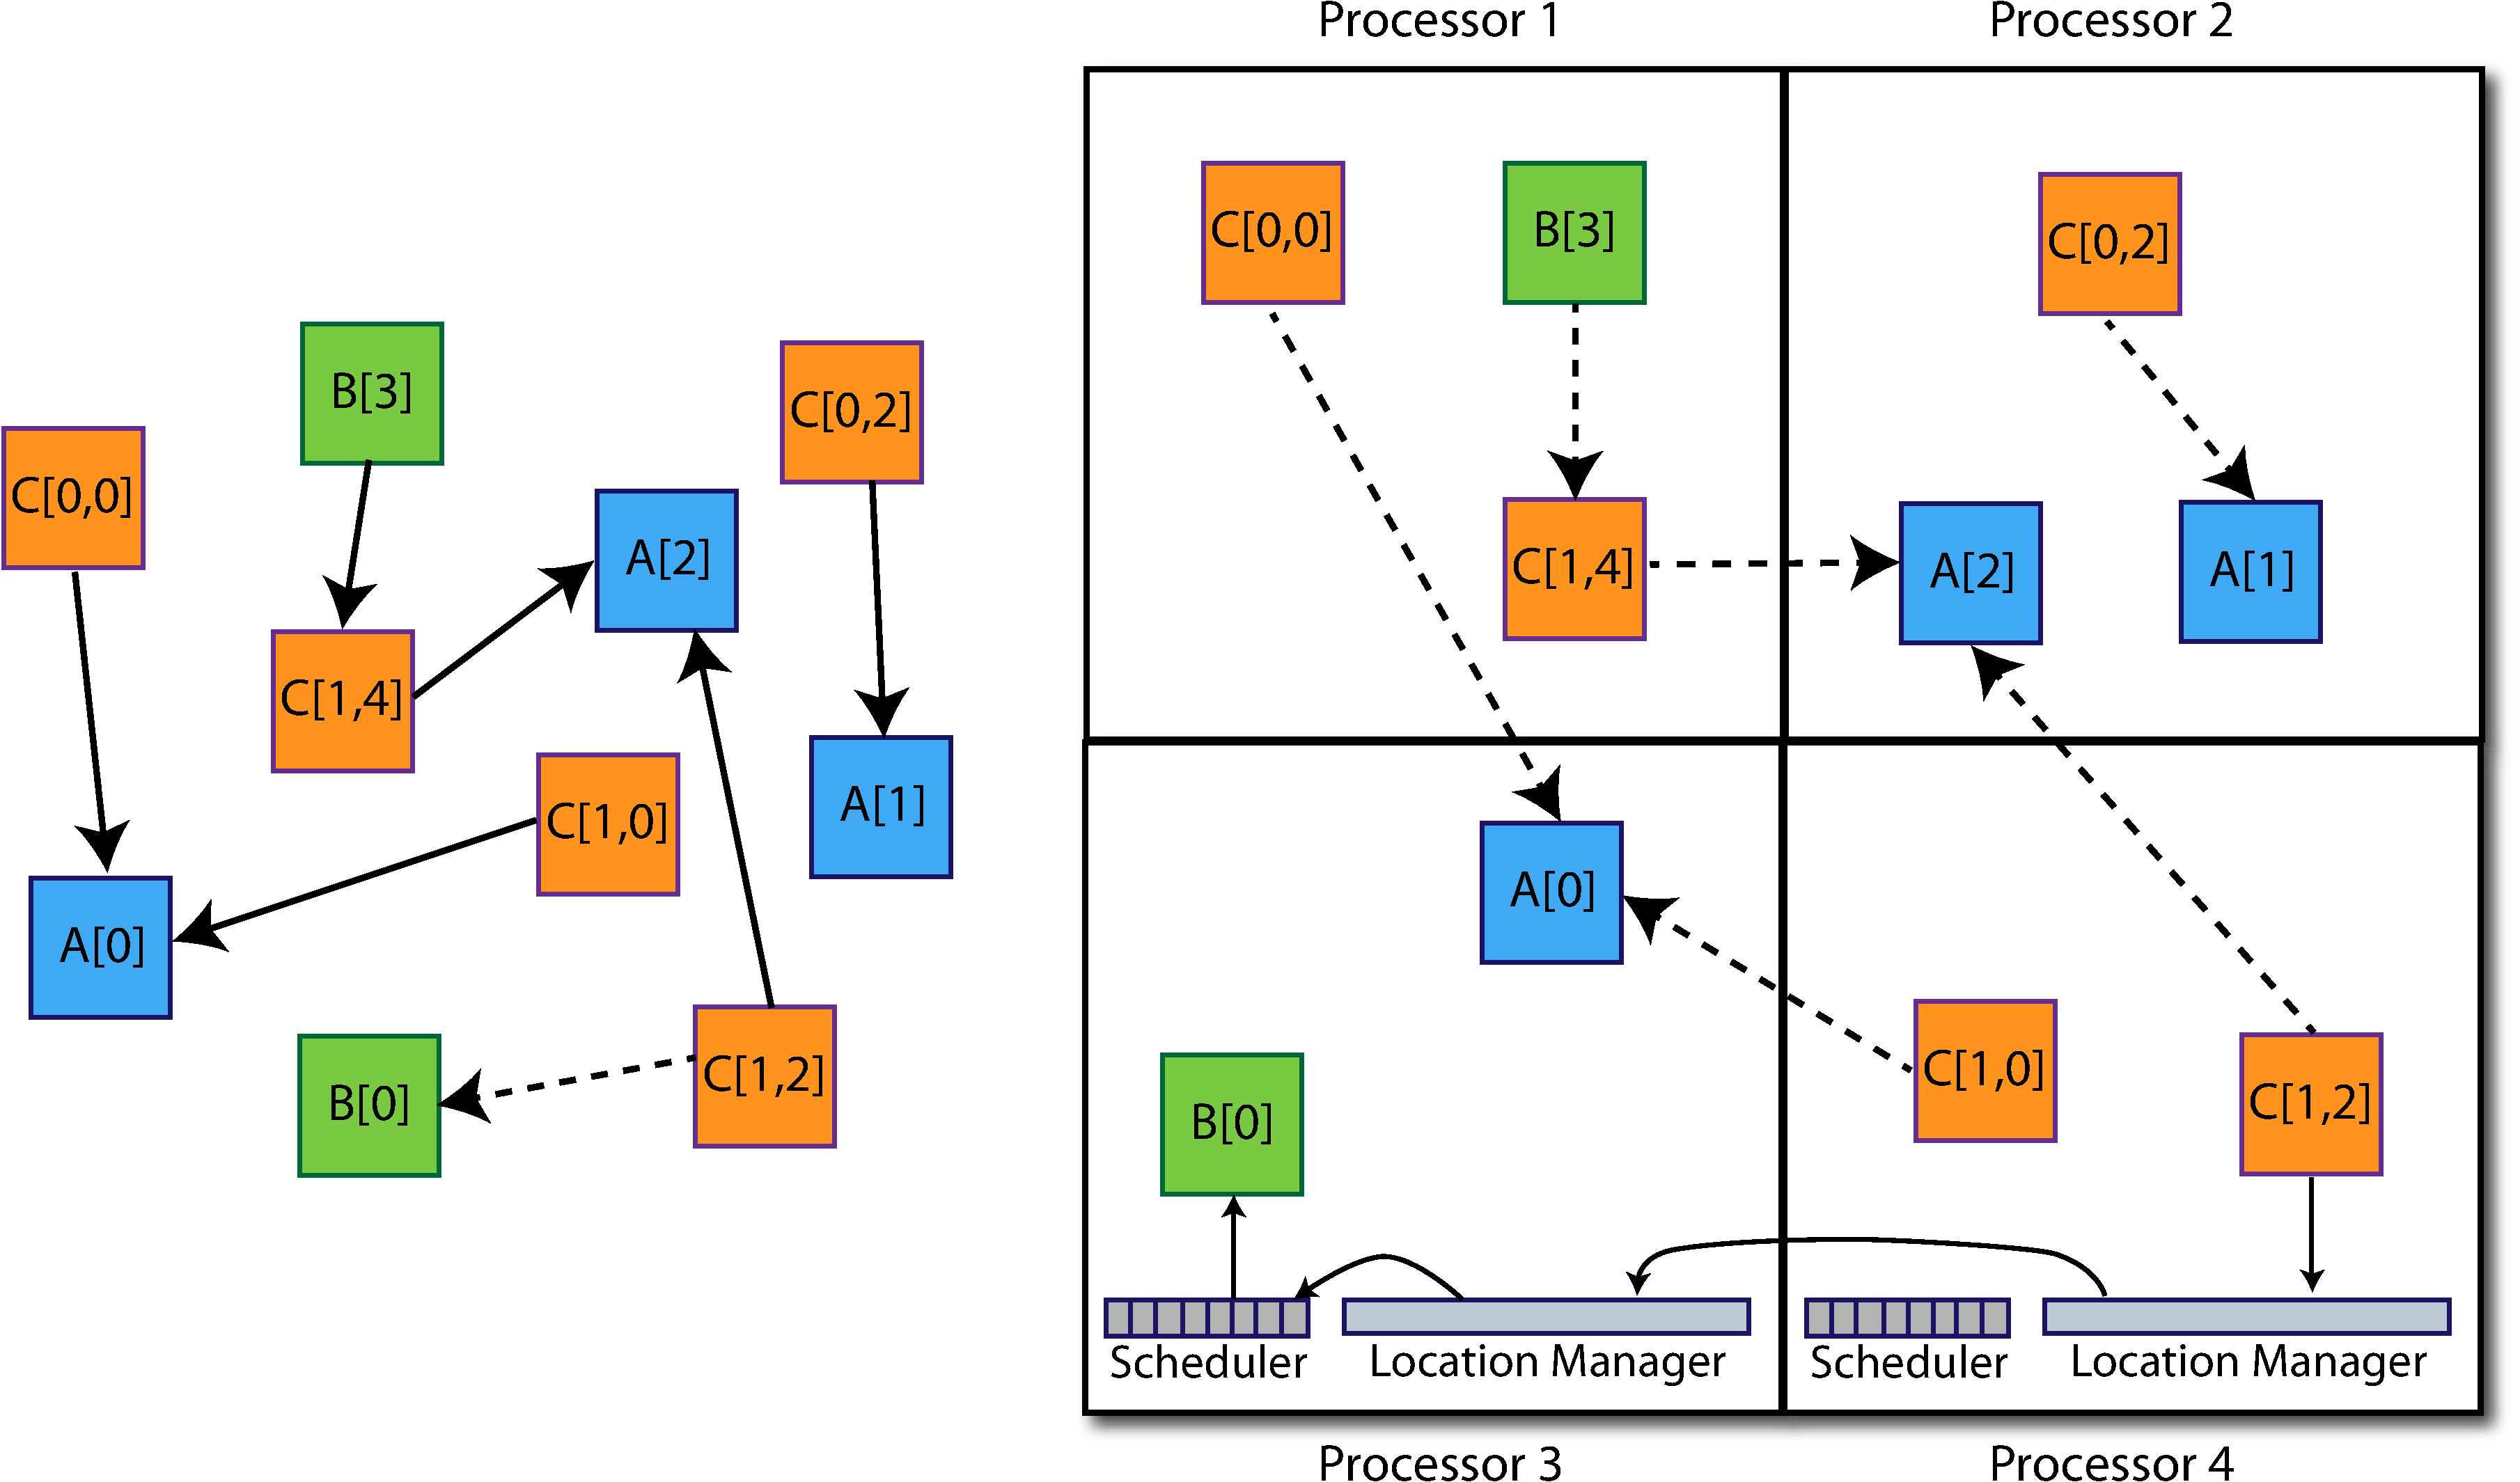
\includegraphics[width=0.9\textwidth]{../figures/elements2.pdf}\end{center}
\end{frame}

\section{Decomposition and Grain Size}
\begin{frame}
\frametitle{Parallel Decomposition}
\framesubtitle{Recap}
\begin{itemize}
\item Data or Task parallelism encoded in objects
\item Object count independent of processors
\item How many objects, then? How big?
\end{itemize}
\end{frame}

\begin{frame}
\frametitle{Parallel Decomposition}
\framesubtitle{Overdecomposition}
Want \emph{several} objects per processor
\begin{itemize}
\item Increase chance that one will have work available
\item Overlap communication of one with computation of another
\item Important for later optimizations
\end{itemize}
\end{frame}

\begin{frame}[fragile]
\frametitle{Parallel Decomposition}
\framesubtitle{Overdecomposition Example: Weather Forecasting in BRAMS}
\begin{itemize}
 \item BRAMS: Brazillian weather code (based on RAMS)
 \item AMPI version (Eduardo Rodrigues, with C. Mendes and J. Panetta)
\end{itemize}
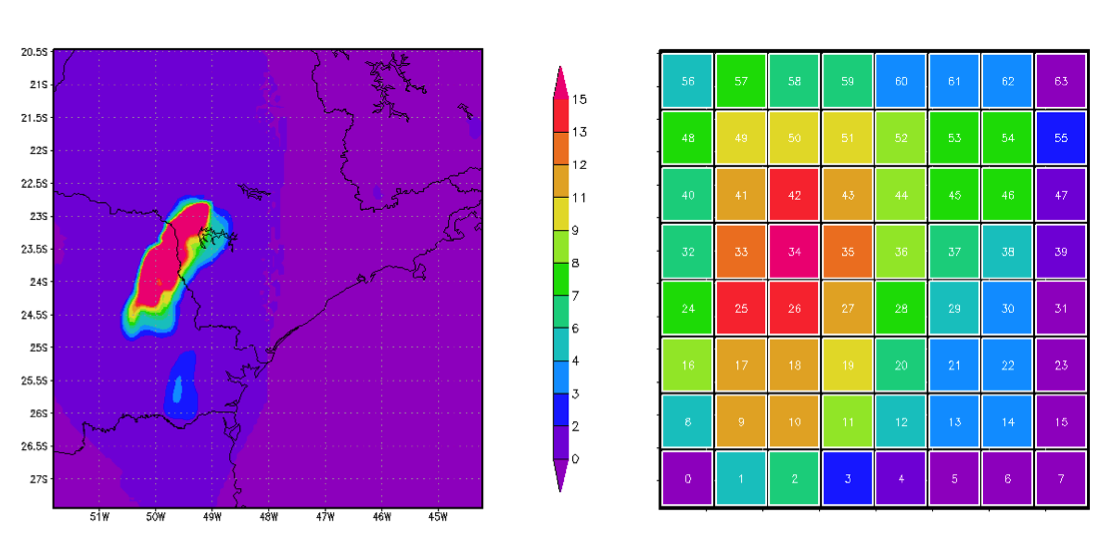
\includegraphics[width=0.9\textwidth]{../figures/bramsVisual.png}
\end{frame}


\begin{frame}[fragile]
\frametitle{Basic Virtualization of BRAMS}
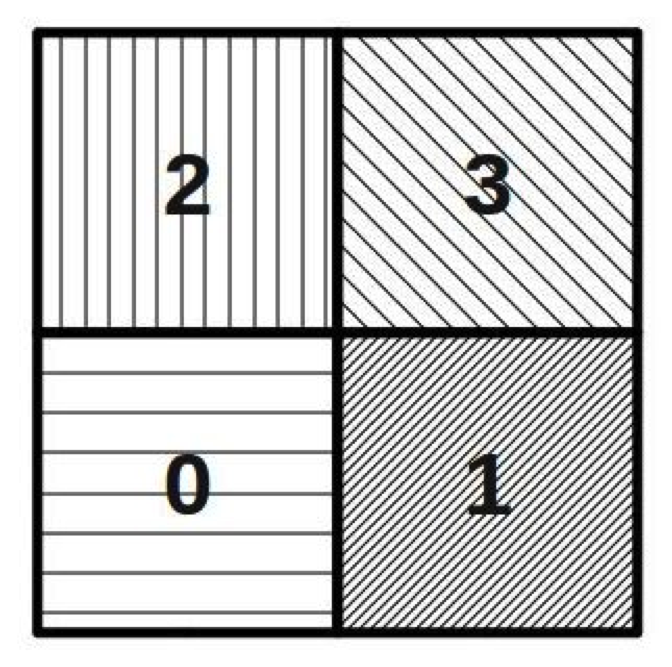
\includegraphics[width=0.5\textwidth]{../figures/bramsNonVirtual.png}
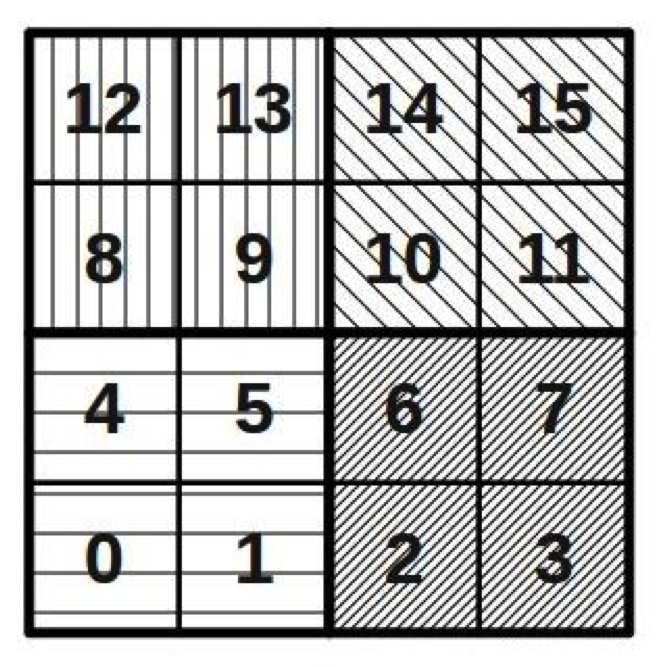
\includegraphics[width=0.5\textwidth]{../figures/bramsVirtual.png}
\end{frame}

\begin{frame}[fragile]
\frametitle{Baseline: 64 objects on 64 processors}
\begin{center}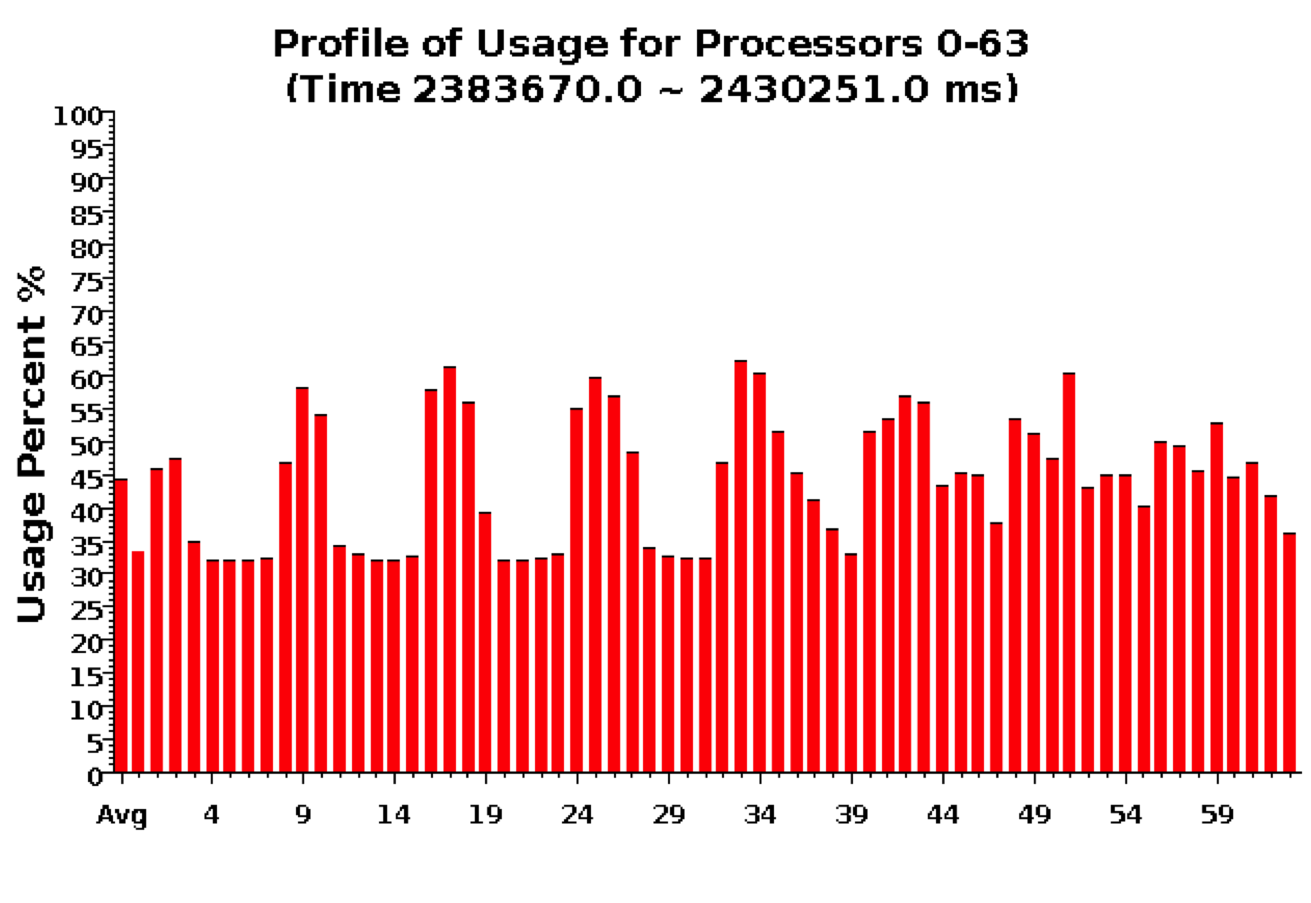
\includegraphics[width=0.9\textwidth]{../figures/usageNonVirtual.png}\end{center}
\end{frame}

\begin{frame}[fragile]
\frametitle{Over-decomposition: 1024 objects on 64 processors}
\framesubtitle{Benefits from communication/computation overlap}
\begin{center}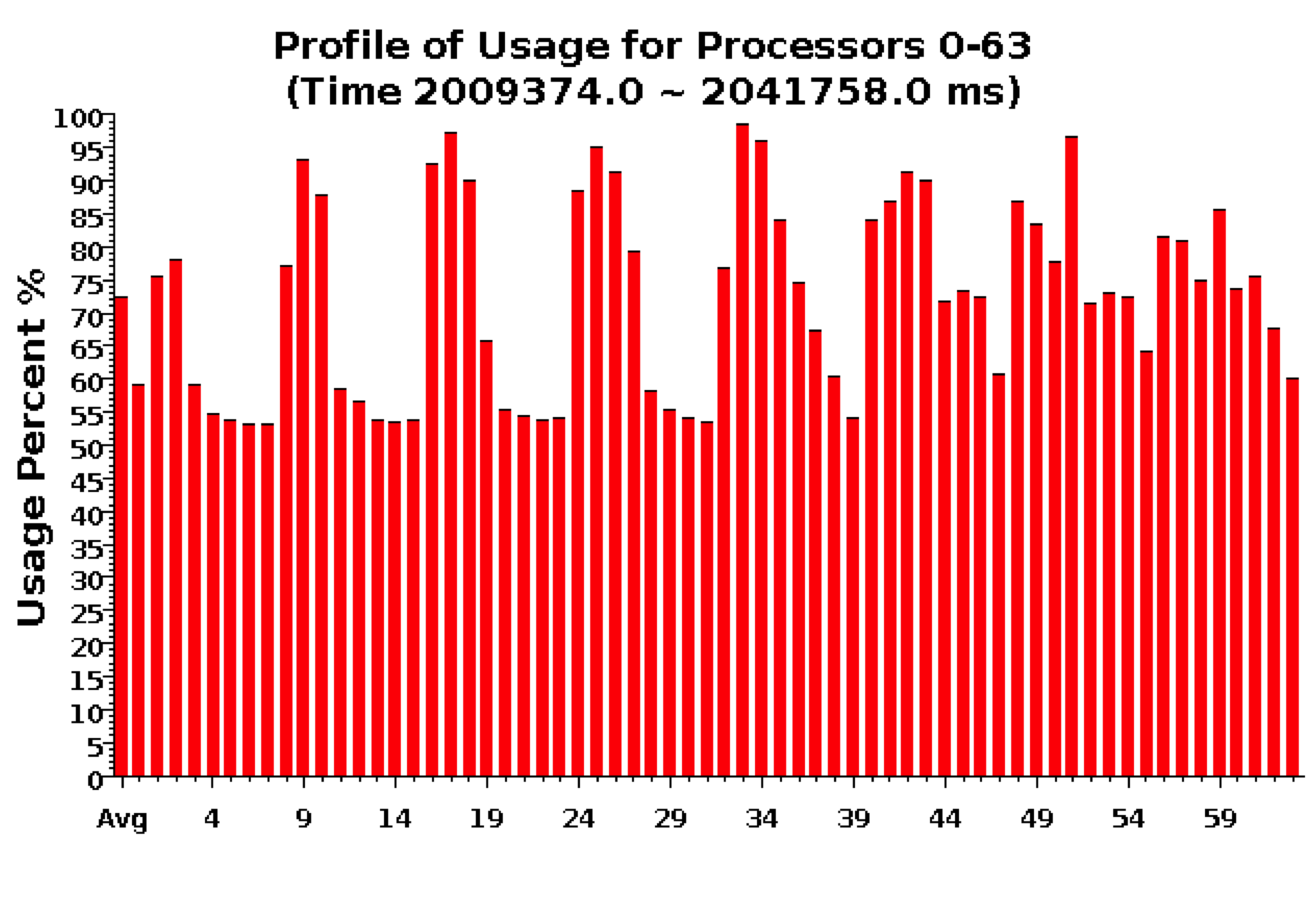
\includegraphics[width=0.9\textwidth]{../figures/usageVirtual.png}\end{center}
\end{frame}


\begin{frame}[fragile]
\frametitle{With Load Balancing: 1024 objects on 64 processors}
\begin{center}
\begin{itemize}
\item No overdecomp (64 threads): 4988 sec
\item Overdecomp into 1024 threads: 3713 sec
\item Load balancing (1024 threads): 3367 sec
\end{itemize}
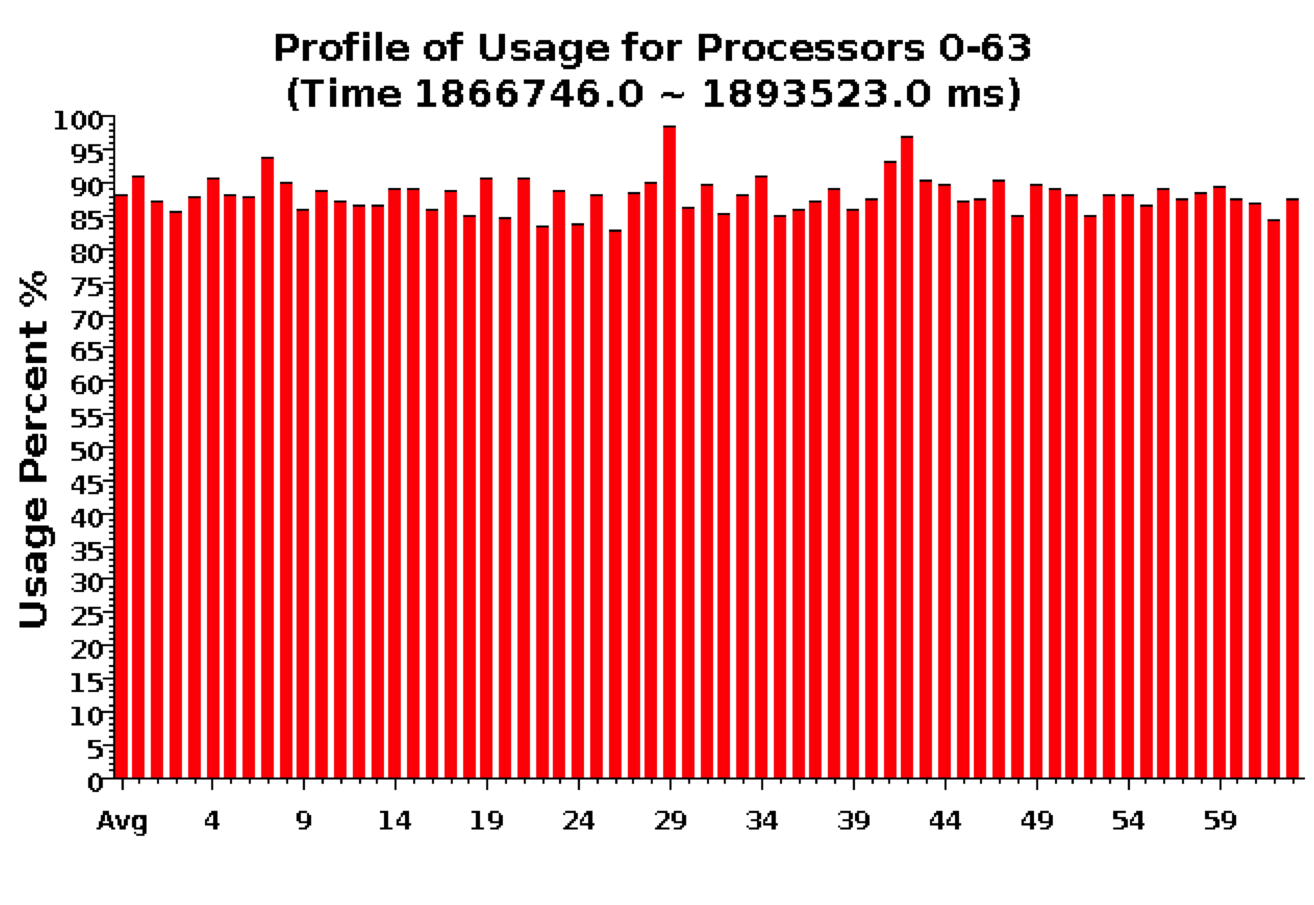
\includegraphics[width=0.8\textwidth]{../figures/usageLB.png}
\end{center}
\end{frame}

\begin{frame}
\frametitle{Grain Size}
  \begin{itemize}
    \item (working) Definition: the amount of computation per potentially
      parallel event (task creation, enqueue/dequeue, messaging,
      locking, etc.)
  \end{itemize}
  \begin{center} 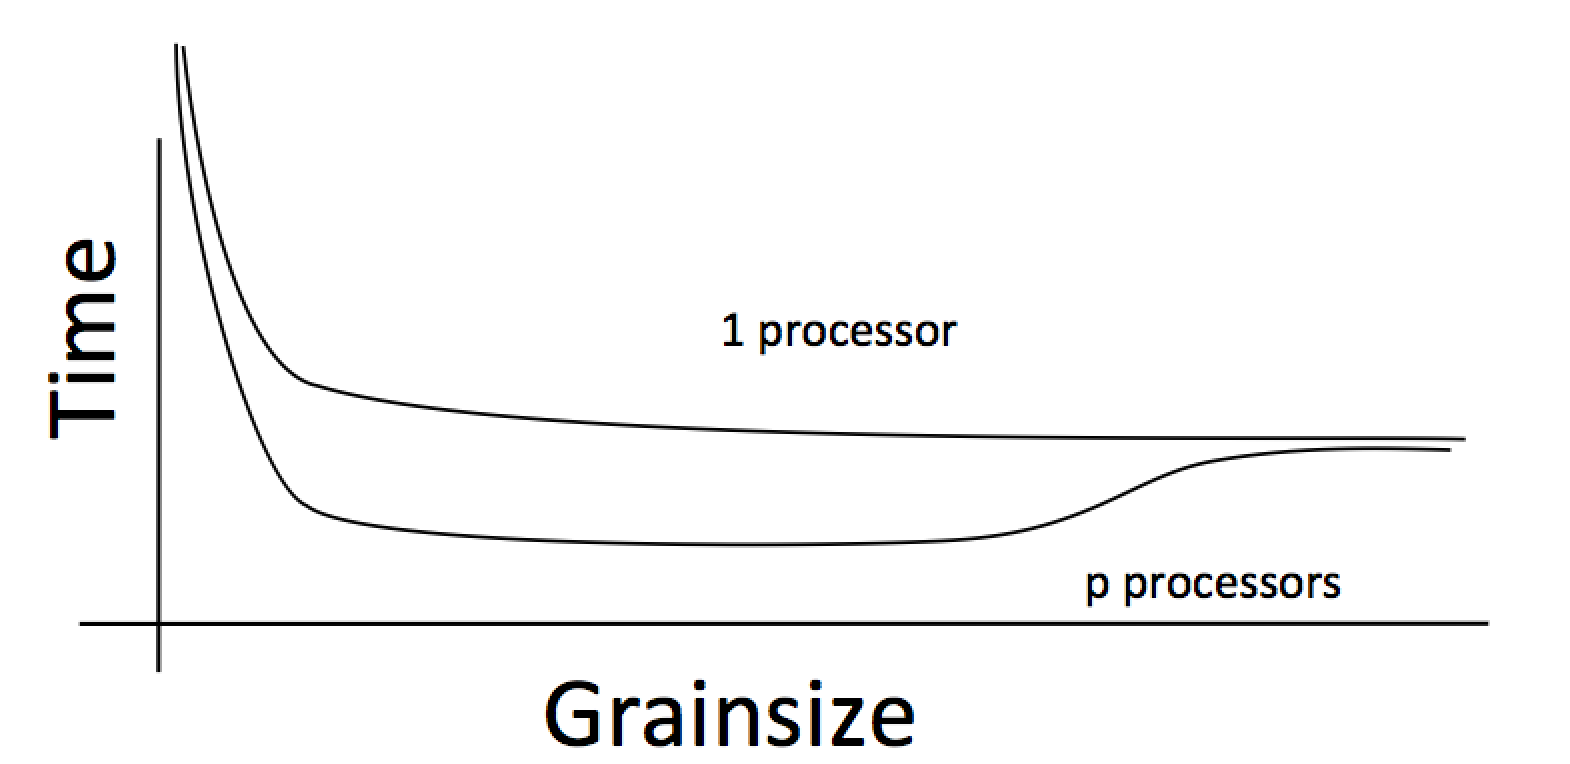
\includegraphics[width=0.7\textwidth]{../figures/grain1.png} \end{center}
\end{frame}

\section{Modularity and Composability}
%\section{Separation of Concerns}
\begin{frame}
\frametitle{Modularity \& Composability}
\begin{itemize}
\item Easy to write code separately and then run it separately
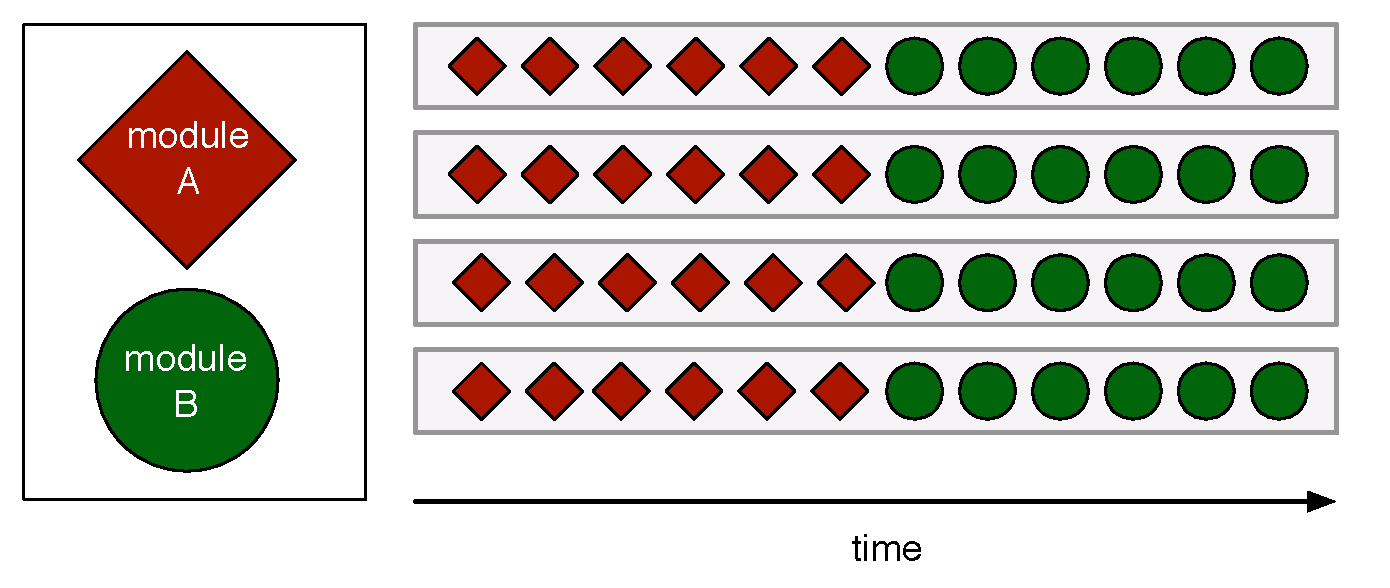
\includegraphics[width=.45\textwidth]{../figures/timeDivision.pdf}
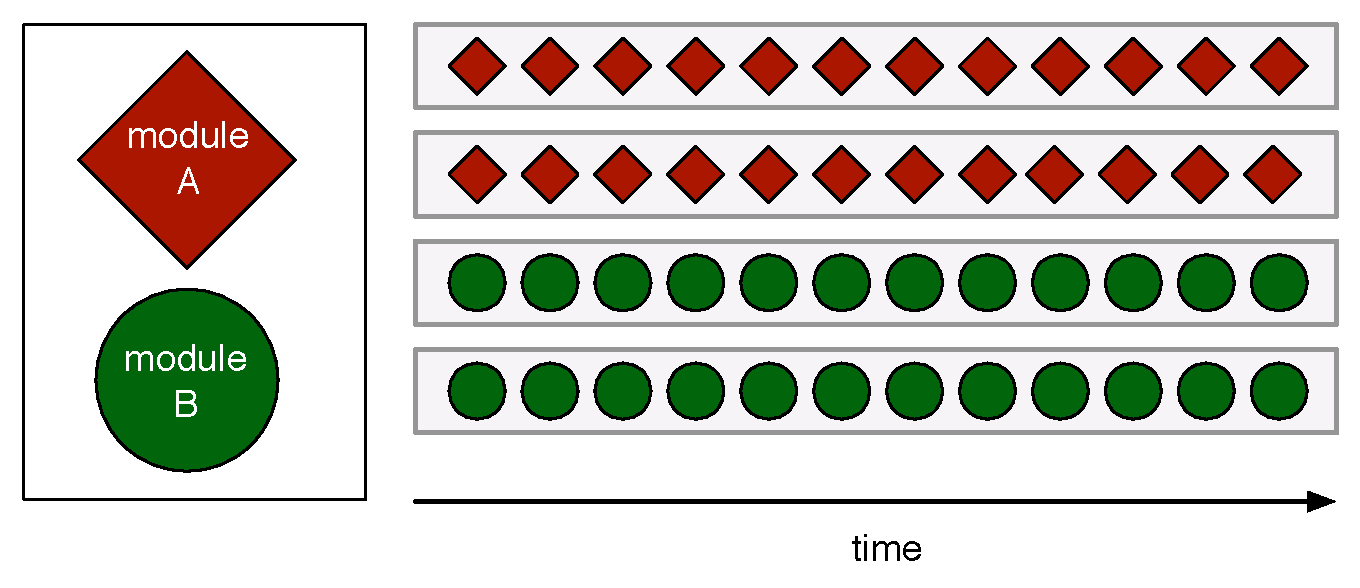
\includegraphics[width=.45\textwidth]{../figures/spaceDivision.pdf}
\item Possible to write code for explicit paralllel composition, interleaving multiple modules
\item Want seamless resource sharing by separate pieces of code
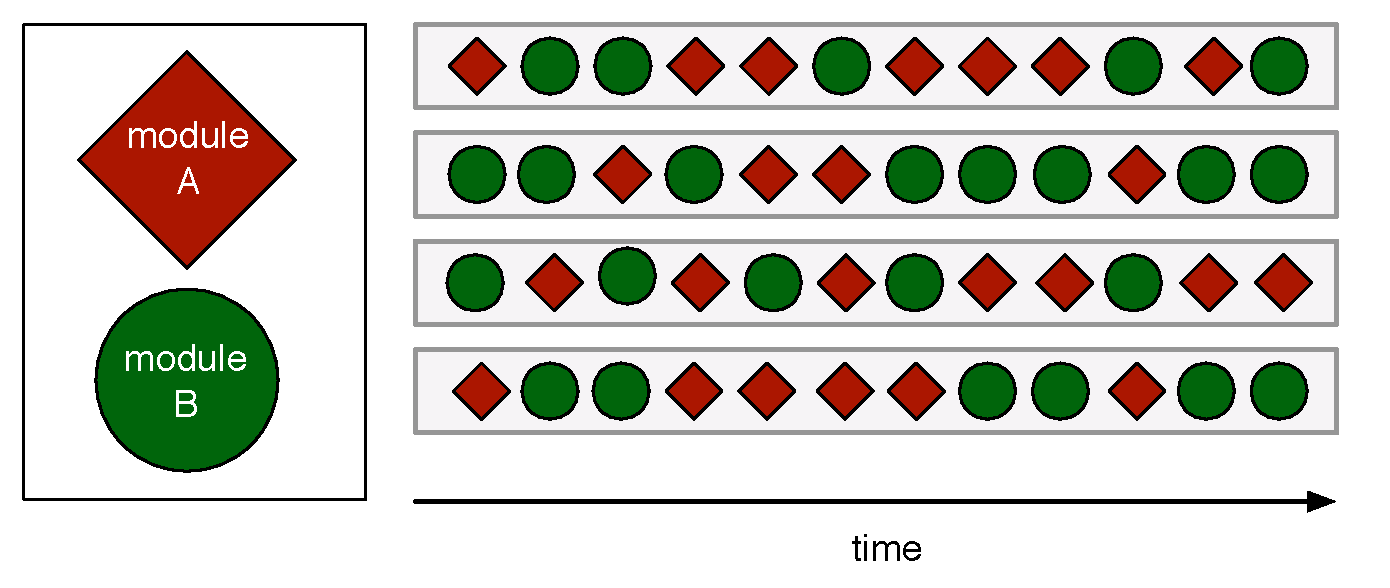
\includegraphics[width=.7\textwidth]{../figures/composition.pdf}
\end{itemize}
\end{frame}

\section{Introspective, Adaptive Runtime System}



\begin{frame}
\frametitle{Load Imbalance}
\begin{itemize}
\item Performance limited by difference between most-loaded processor and overall average.\\
\only<1>{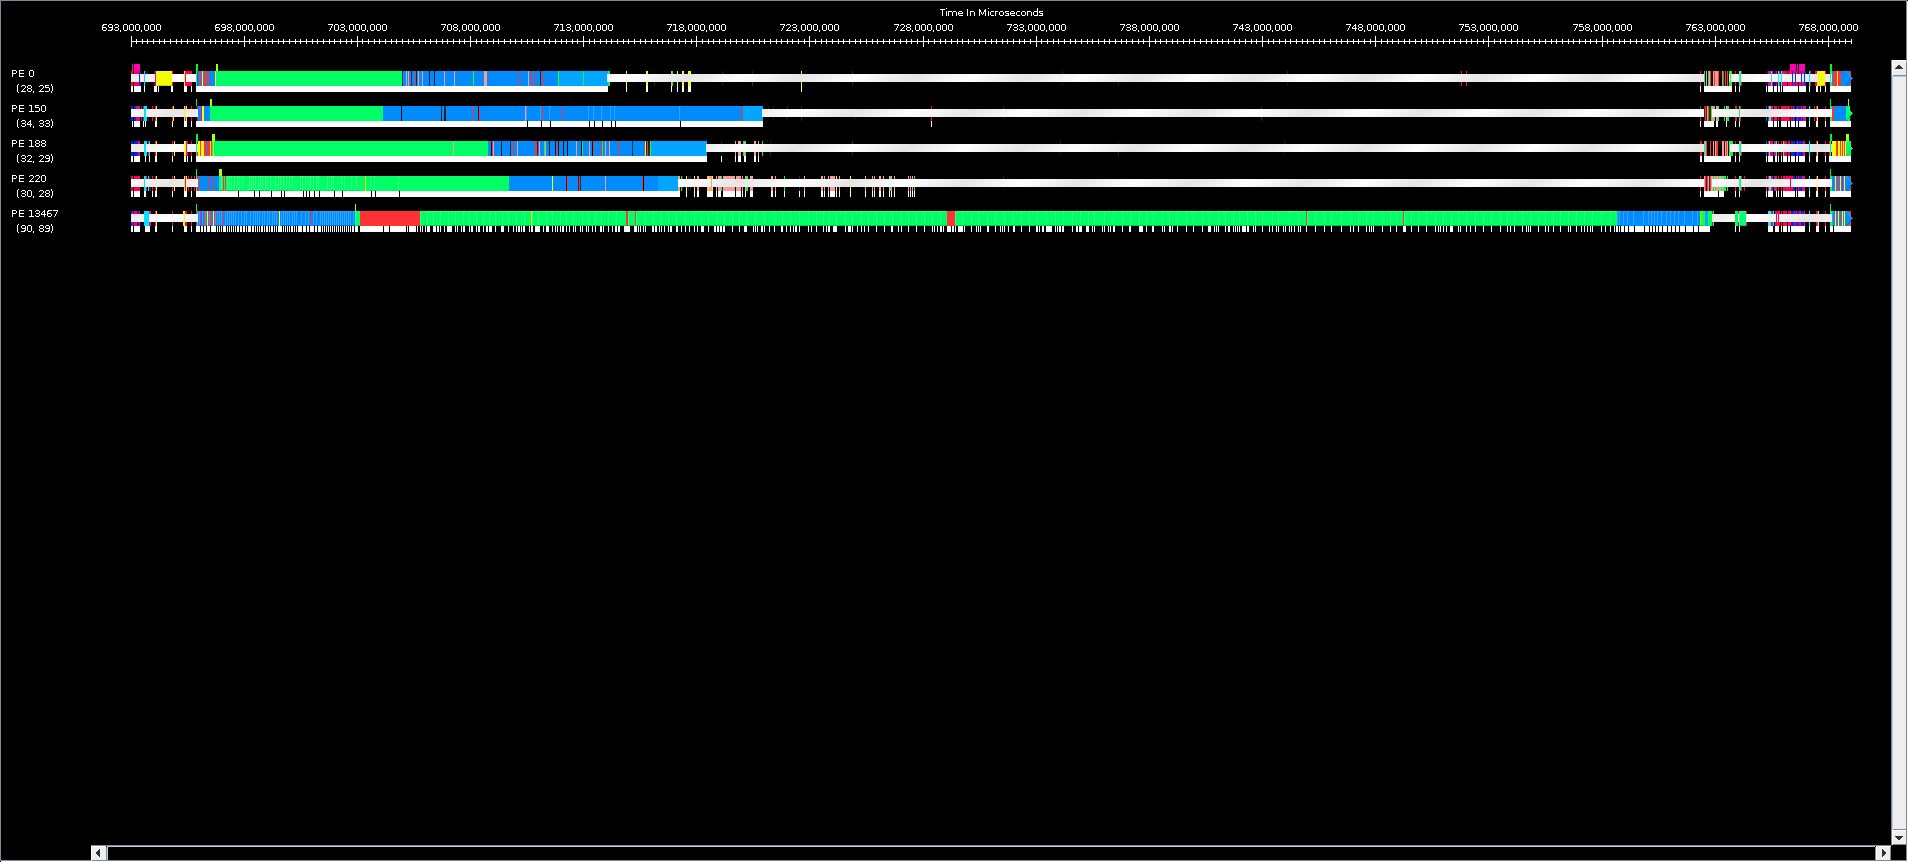
\includegraphics[width=0.8\textwidth]{../figures/changa_imbalance.png}}
\pause
\item Causes vary in severity, time scale, nature
\pause
\item Response must suit causes, other application concerns, system scale
\end{itemize}
\end{frame}


\begin{frame}[fragile]
\frametitle{With Load Balancing: 1024 objects on 64 processors}
\begin{center}
\begin{itemize}
\item No overdecomp (64 threads): 4988 sec
\item Overdecomp into 1024 threads: 3713 sec
\item<2-> Load balancing (1024 threads): 3367 sec
\end{itemize}
\includegraphics<1>[width=0.9\textwidth]{../figures/usageVirtual.png}
\includegraphics<2>[width=0.8\textwidth]{../figures/usageLB.png}
\end{center}
\end{frame}


\begin{frame}
\frametitle{Load Balancing Adaptive Mesh Refinement for solving PDEs}
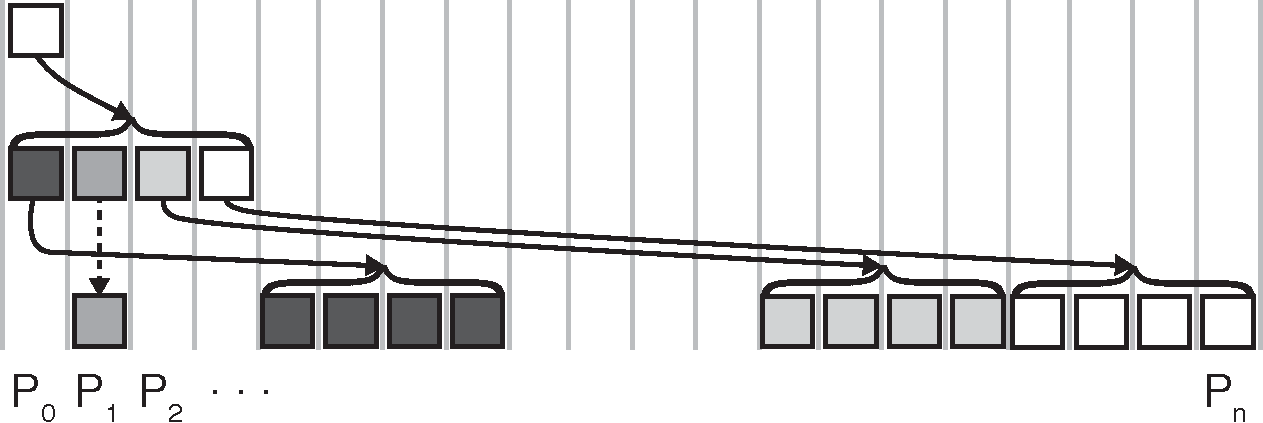
\includegraphics[width=0.9\textwidth]{../figures/amr_mapping.pdf}\\
Load changes gradually and incrementally, suggesting localized strategies
\end{frame}


\begin{frame}
\frametitle{Load Balancing Adaptive Mesh Refinement for solving PDEs}
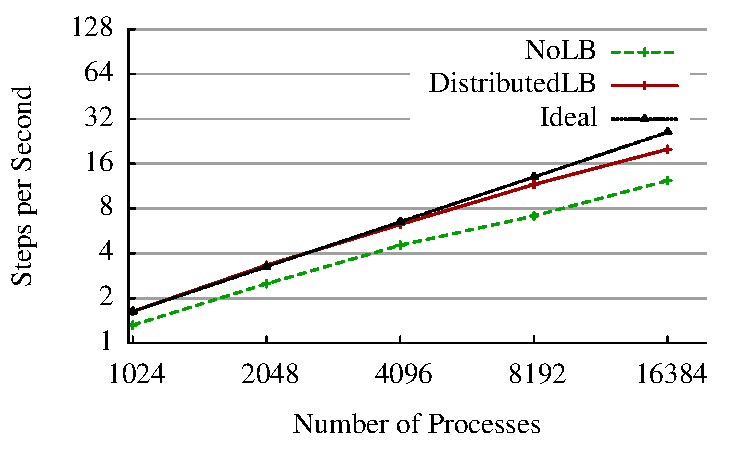
\includegraphics[width=0.9\textwidth]{../figures/amr_scaling_distlb.pdf}
\end{frame}


\begin{frame}[fragile]
\frametitle{Load Imbalance: Crack Propagation}
\begin{columns}
\begin{column}{0.5\textwidth}
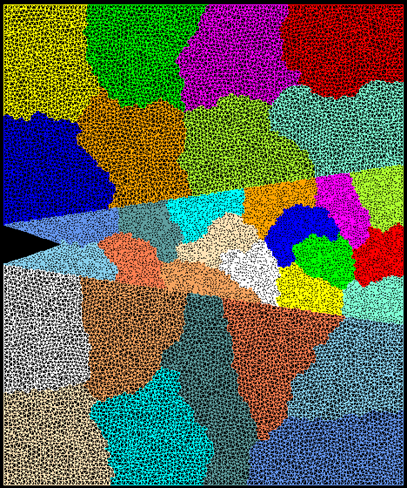
\includegraphics[width=\textwidth]{../figures/chunkGraph16}
\end{column}
\begin{column}{0.5\textwidth}
Decomposition into 16 chunks using Metis. The middle area contains cohesive elements.

As computation progresses, crack propagates, and new elements are added, leading to more complex computations in some chunks

Picture: S. Breitenfeld and P. Geubelle
\end{column}
\end{columns}
\end{frame}


\begin{frame}[fragile]
\frametitle{Load Balancing Crack Propagation}
\begin{centering}
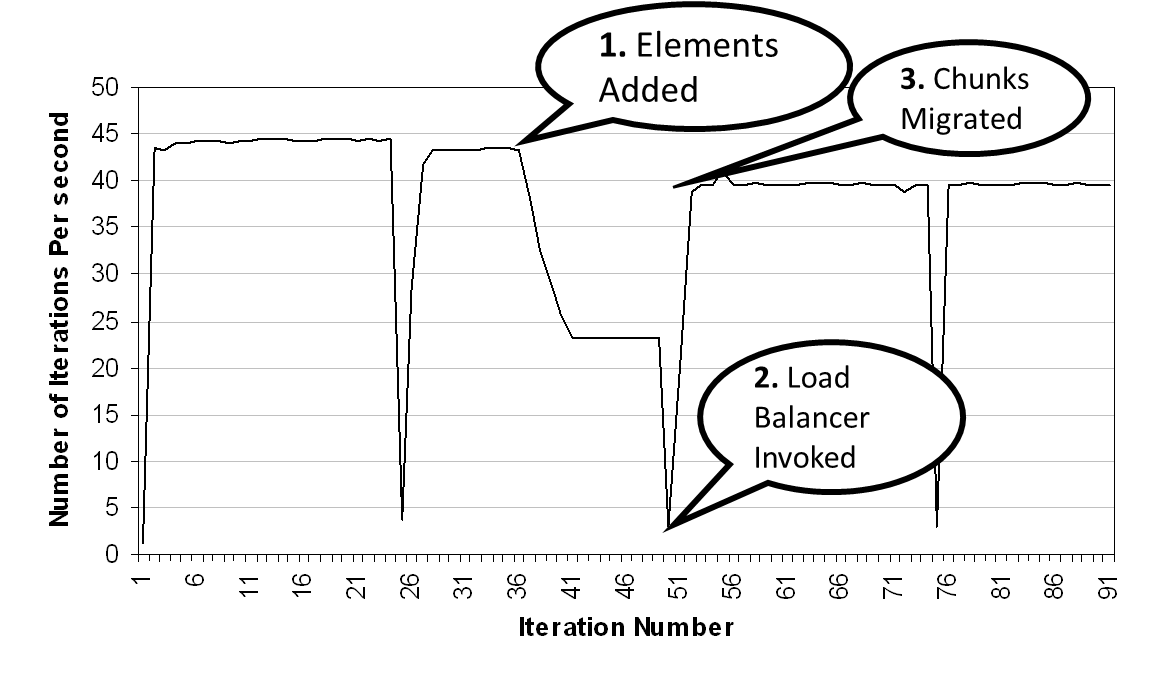
\includegraphics[width=0.8\textwidth]{../figures/LButilizationCrackPropWithAnnotation}
\end{centering}
\begin{block}{Sudden, severe shift in load suggests comprehensive rebalancing}
Link-time: \texttt{-balancer GreedyLB} or \texttt{-balancer MetisLB} \\
Run-time: \texttt{+balancer FooLB}
\end{block}
\end{frame}


\begin{frame}
\frametitle{Load Imbalance: Adaptive Response}
\begin{itemize}
\item When to run load balancer? \pause When imbalance hurts (worse than the cost)!
\end{itemize}
\only<2>{
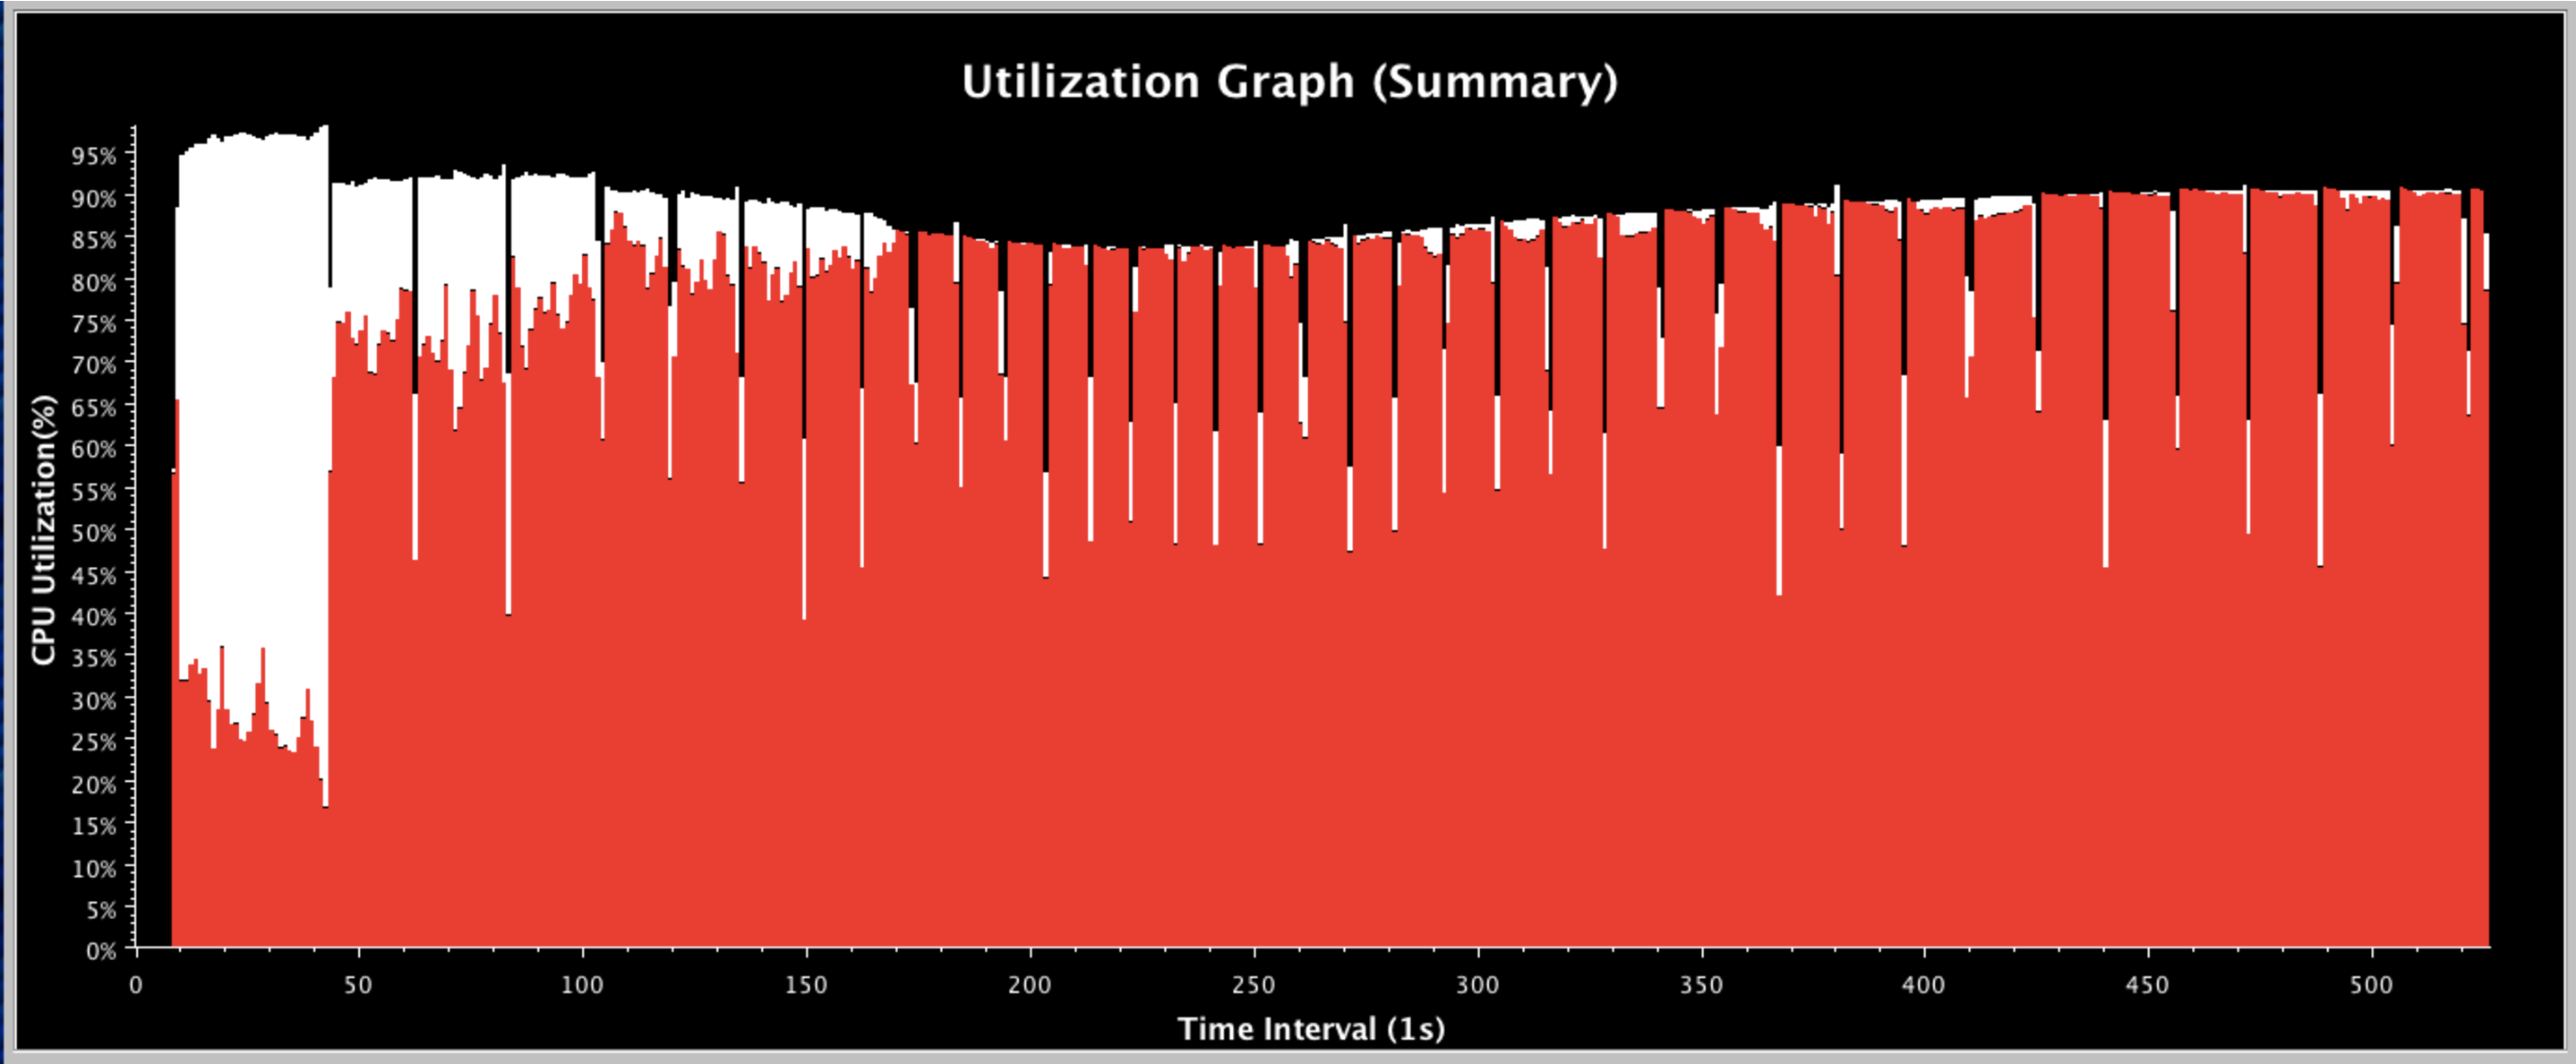
\includegraphics[width=0.5\textwidth]{../figures/figs_frac_titan_lb300_vp4k_64_proj.pdf}
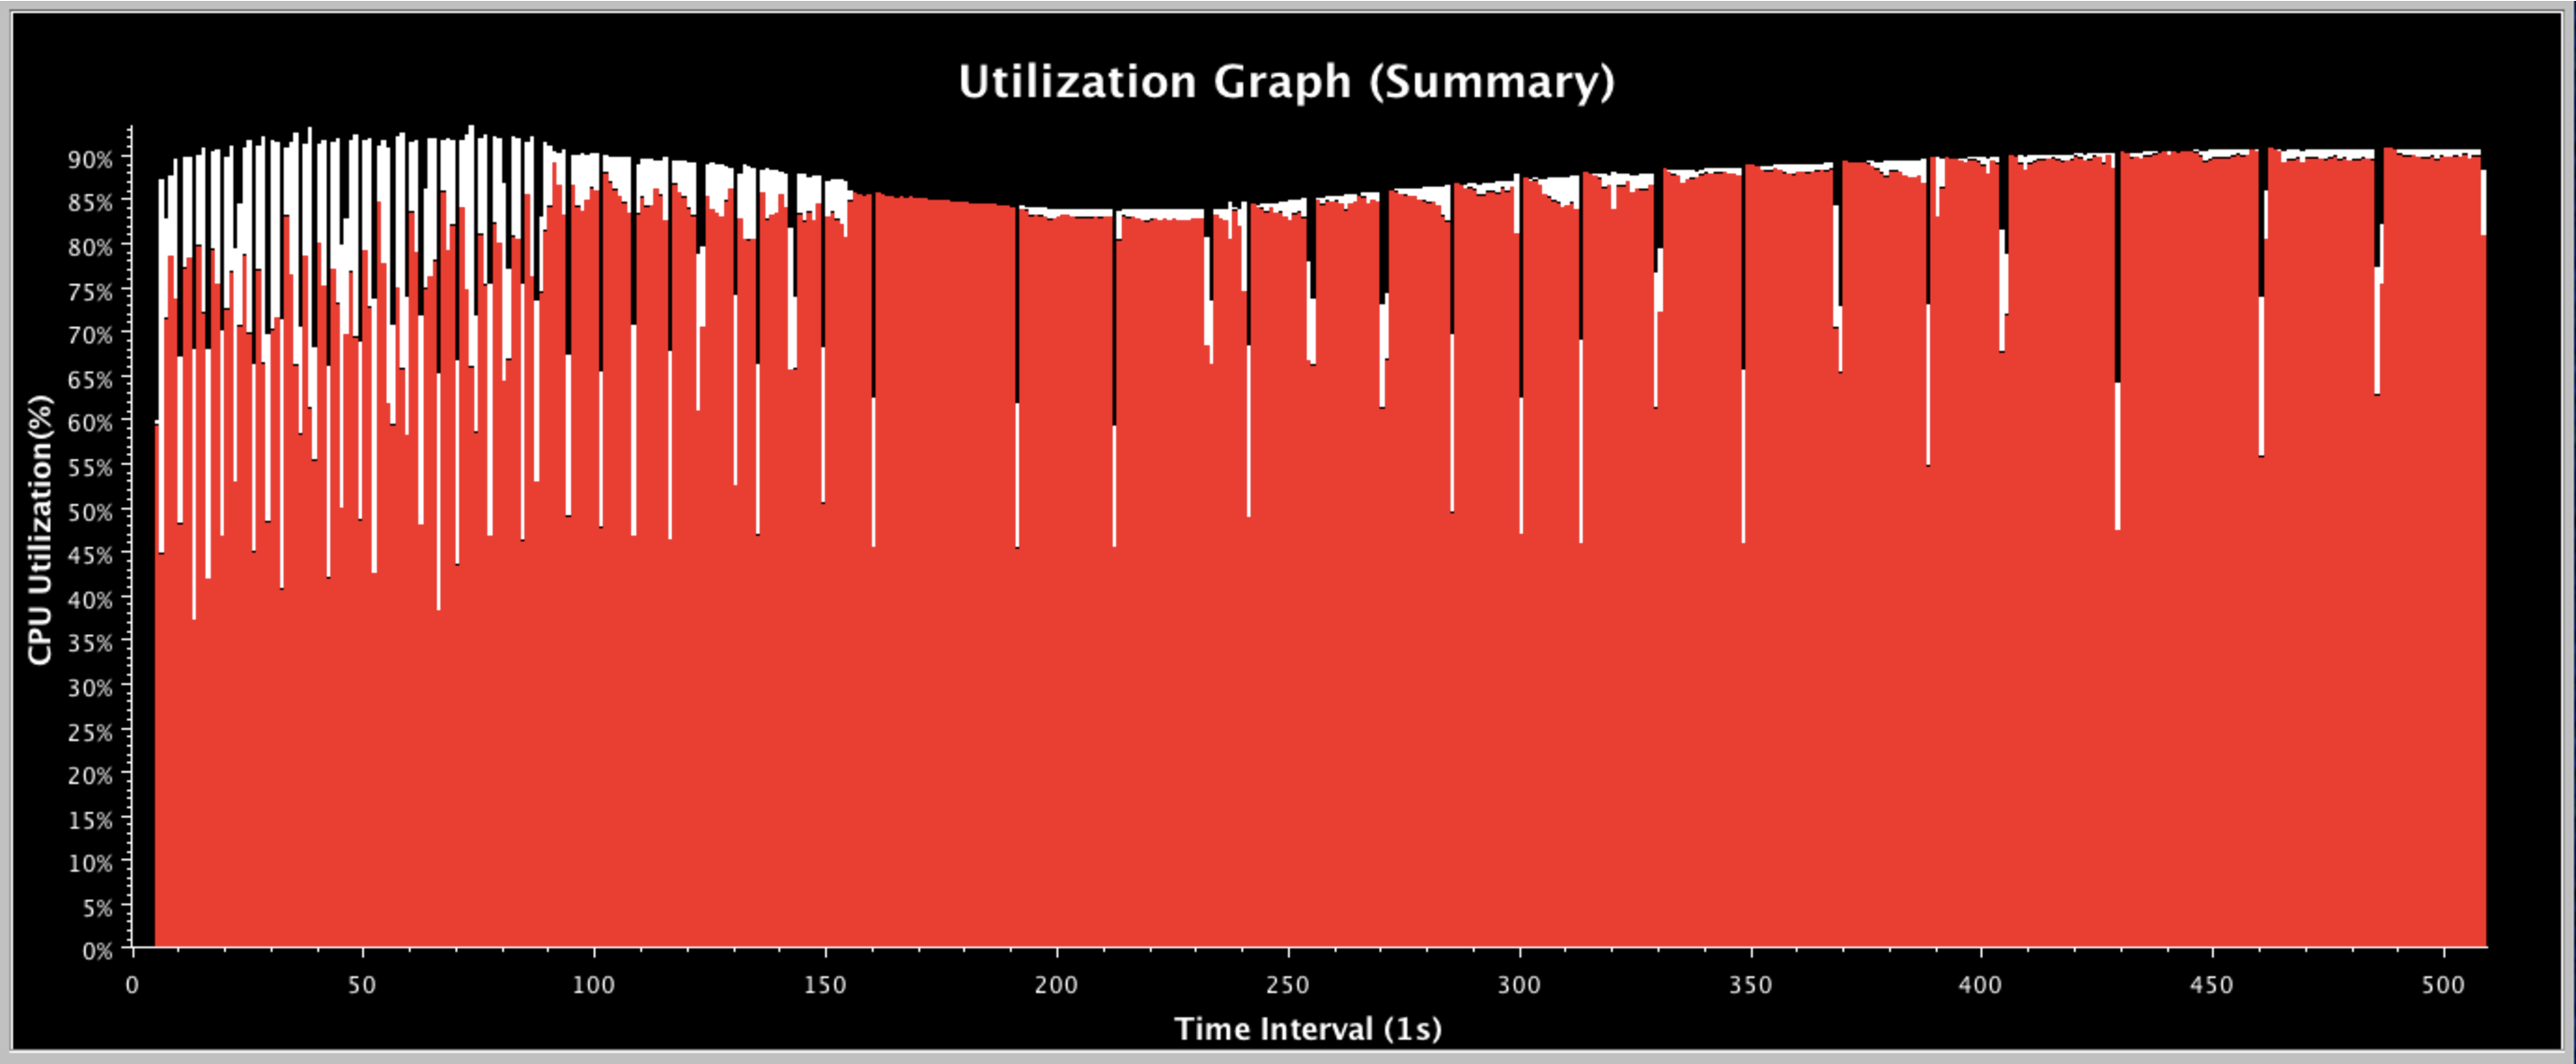
\includegraphics[width=0.5\textwidth]{../figures/figs_frac_titan_meta_vp4k_64_proj.pdf}
\begin{block}{How to activate?}
\texttt{./pgm argsA argsB argsC +MetaLB}
\end{block}
}
\end{frame}

\begin{frame}
\frametitle{Load Imbalance: Adaptive Response}
\begin{itemize}
\item When to run load balancer? When imbalance hurts (worse than the cost)!
\item When to allow migration? \pause When imbalance hurts (worse than the cost)!
\end{itemize}
\only<2>{
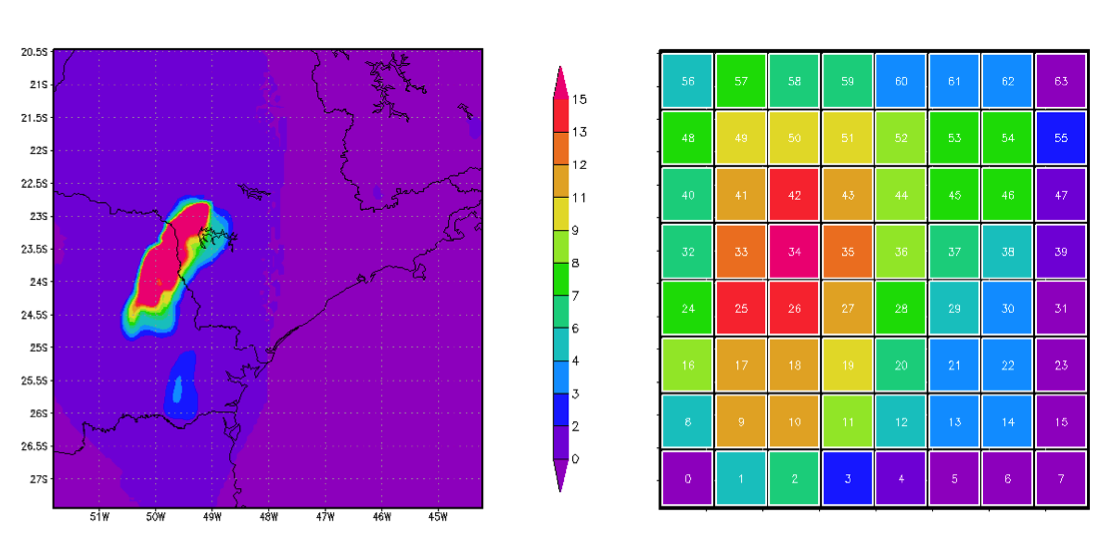
\includegraphics[width=0.9\textwidth]{../figures/bramsVisual.png}
}
\end{frame}

\begin{frame}
\frametitle{Power, Energy, and Heat}
\framesubtitle{Motivations}
\begin{itemize}
\item Reduce direct costs of execution - cumulative machine energy, cooling energy from start to finish
\item Reduce capital costs - transformers, chillers
\item Improve reliability
\item Improve user experience - fan noise, ambient heat, battery life
\end{itemize}
\end{frame}

\begin{frame}[t]
\frametitle{Power, Energy, and Heat}
\begin{block}{Established Technique}
Set temperature threshold, periodic DVFS to enforce
\end{block}
\begin{itemize}
\item Slower clocks can hurt performance
\item Load balance to compensate
\end{itemize}
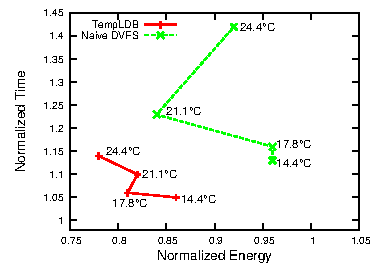
\includegraphics[width=0.3\textwidth]{../figures/ft_par.pdf}
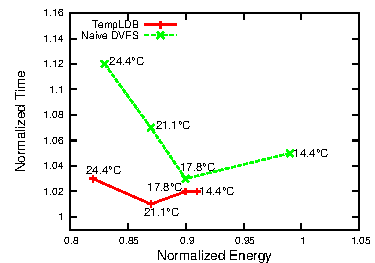
\includegraphics[width=0.3\textwidth]{../figures/jacobi_par.pdf}
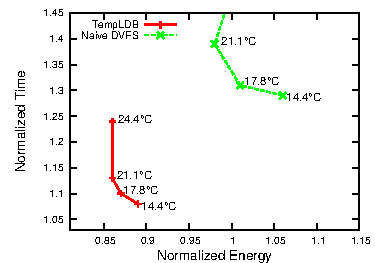
\includegraphics[width=0.3\textwidth]{../figures/wave_par_bk.pdf}
\pause
\begin{block}{Upcoming Technique}
Set power threshold on newer Intel CPUs, load balance as overloads appear
\end{block}
\end{frame}



\input{ft}
\section{Scalability}
\begin{frame}
\frametitle{Contagion and Information Spread: CharmEpiSimDemics}
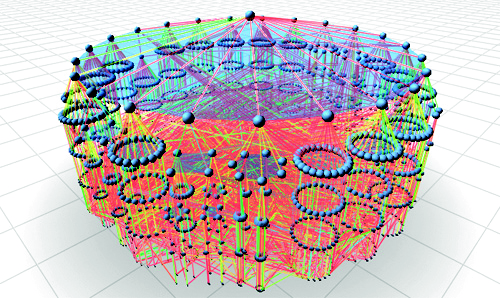
\includegraphics[width=\textwidth]{../figures/contagion.png}
\end{frame}


\begin{frame}
\frametitle{Contagion and Information Spread: CharmEpiSimDemics}
\begin{center}
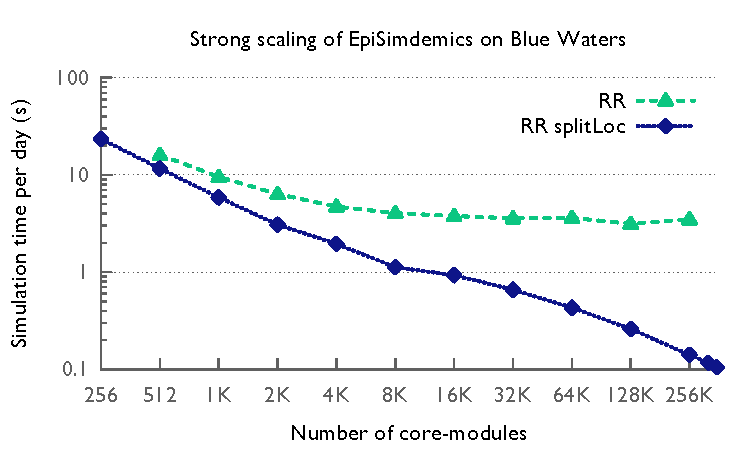
\includegraphics[width=0.9\textwidth]{../figures/simdemics_strong_scaling.pdf}
\end{center}
\end{frame}


\begin{frame}
\frametitle{JetAlloc}
%
\begin{itemize}
\item
\end{itemize}
%
%\includegraphics{../figures/}
\end{frame}

\begin{frame}
\frametitle{kd-tree construction on multicores}
\framesubtitle{4 socket, 40 core intel xeon E7-4860 at 2.27GHz}
\includegraphics<1>[height=\textheight]{../figures/kdtree/speedup_8.pdf}
\includegraphics<2>[height=\textheight]{../figures/kdtree/speedup_15.pdf}
\end{frame}


\begin{frame}
\frametitle{Numerical Linear Algebra: Dense LU Factorization}
\begin{center}
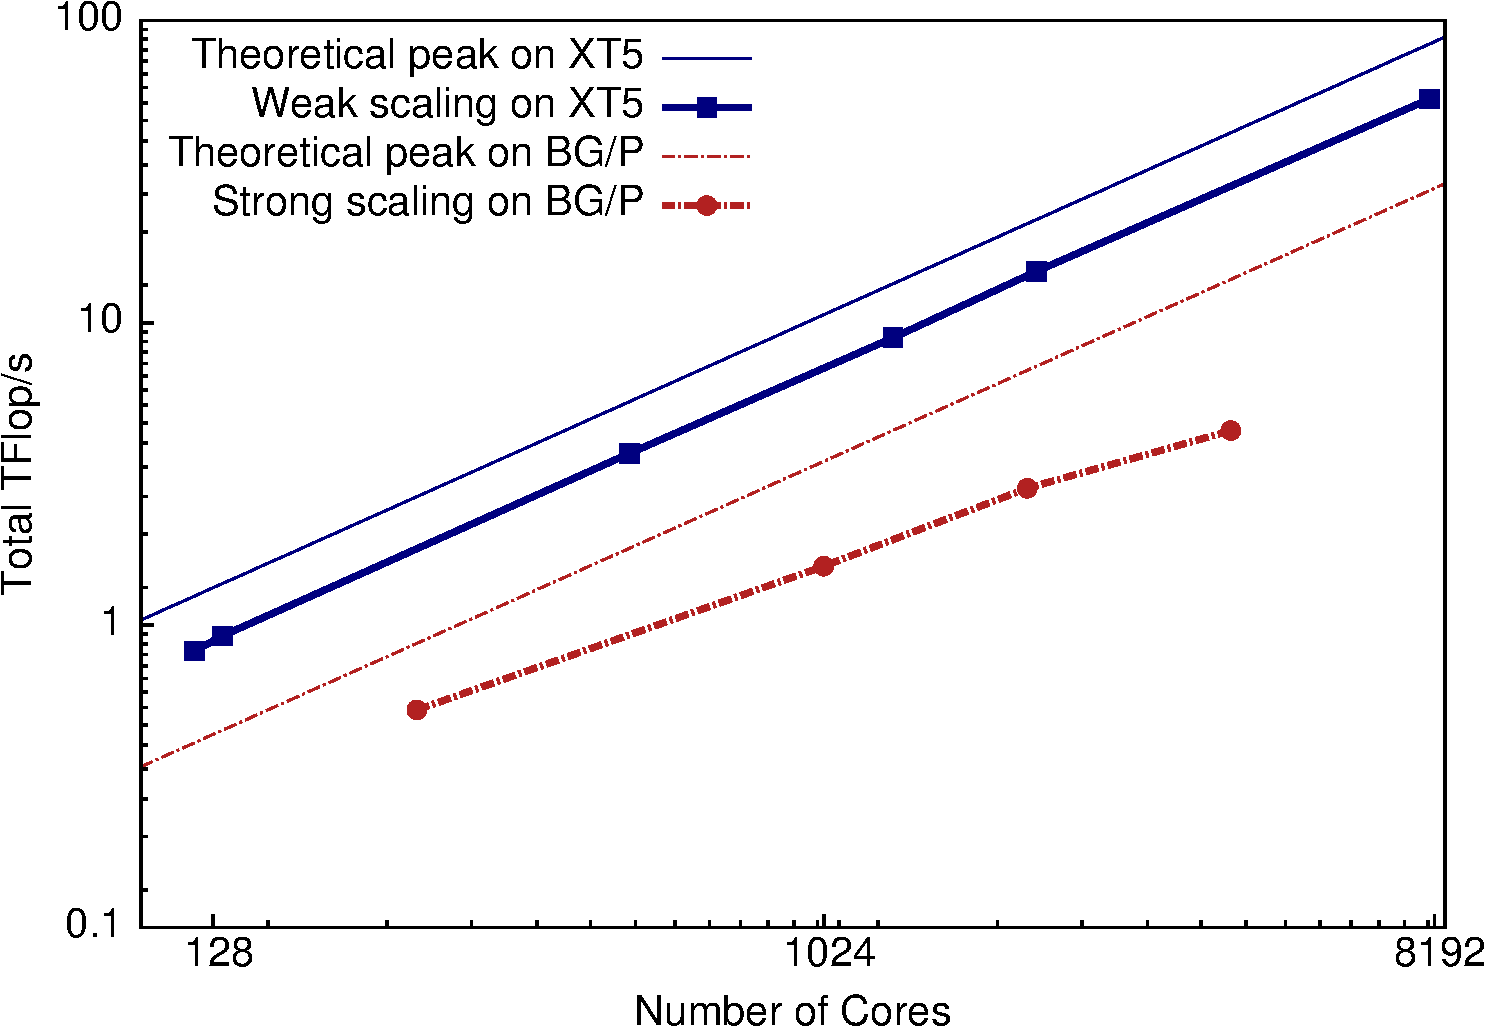
\includegraphics[width=0.9\textwidth]{../figures/charmlu_scaling.pdf}
\end{center}
\end{frame}


\section{Tooling}
\begin{frame}
  \frametitle{Performance Analysis Using Projections}
  \begin{block}{Instrumentation and measurement during program execution}
    \begin{itemize}
        \item Easy setup: just modify link options
        \item Easy setup: data is generated automatically during run
        \item User events can be easily inserted as needed
    \end{itemize}
  \end{block}
  \begin{block}{Visualization and analysis client}
    \begin{itemize}
        \item Scalable: analyze execution traces for 100s of thousands of cores 
        \item Rich feature set: time profile, time lines, usage profile, histograms, outliers etc
        \item Detect performance problems: load imbalance, grain size, communication bottleneck, etc 
    \end{itemize}
  \end{block}
\end{frame}


\begin{frame}{Time Profile}
 \includegraphics<1>[width=0.9\textwidth]{../figures/prj1M8KTimeprofile.png}
\end{frame}

\begin{frame}{Extrema Tool for Least Idle Processors}
\includegraphics<1>[width=0.9\textwidth]{../figures/prj1M8KExtrema.png}
\end{frame}

\begin{frame}{Time Lines with Message Back Tracing}
\centering
\includegraphics<1>[width=0.9\textwidth]{../figures/prj1M8KTimeline.png}
\end{frame}


\begin{frame}{Communication over Time for all Processors}
 \includegraphics<1>[width=0.9\textwidth]{../figures/prj1M8KCommtime.png}
\end{frame}


\begin{frame}[fragile]
  \frametitle{Debugging \charm applications using CharmDebug}
  \begin{center}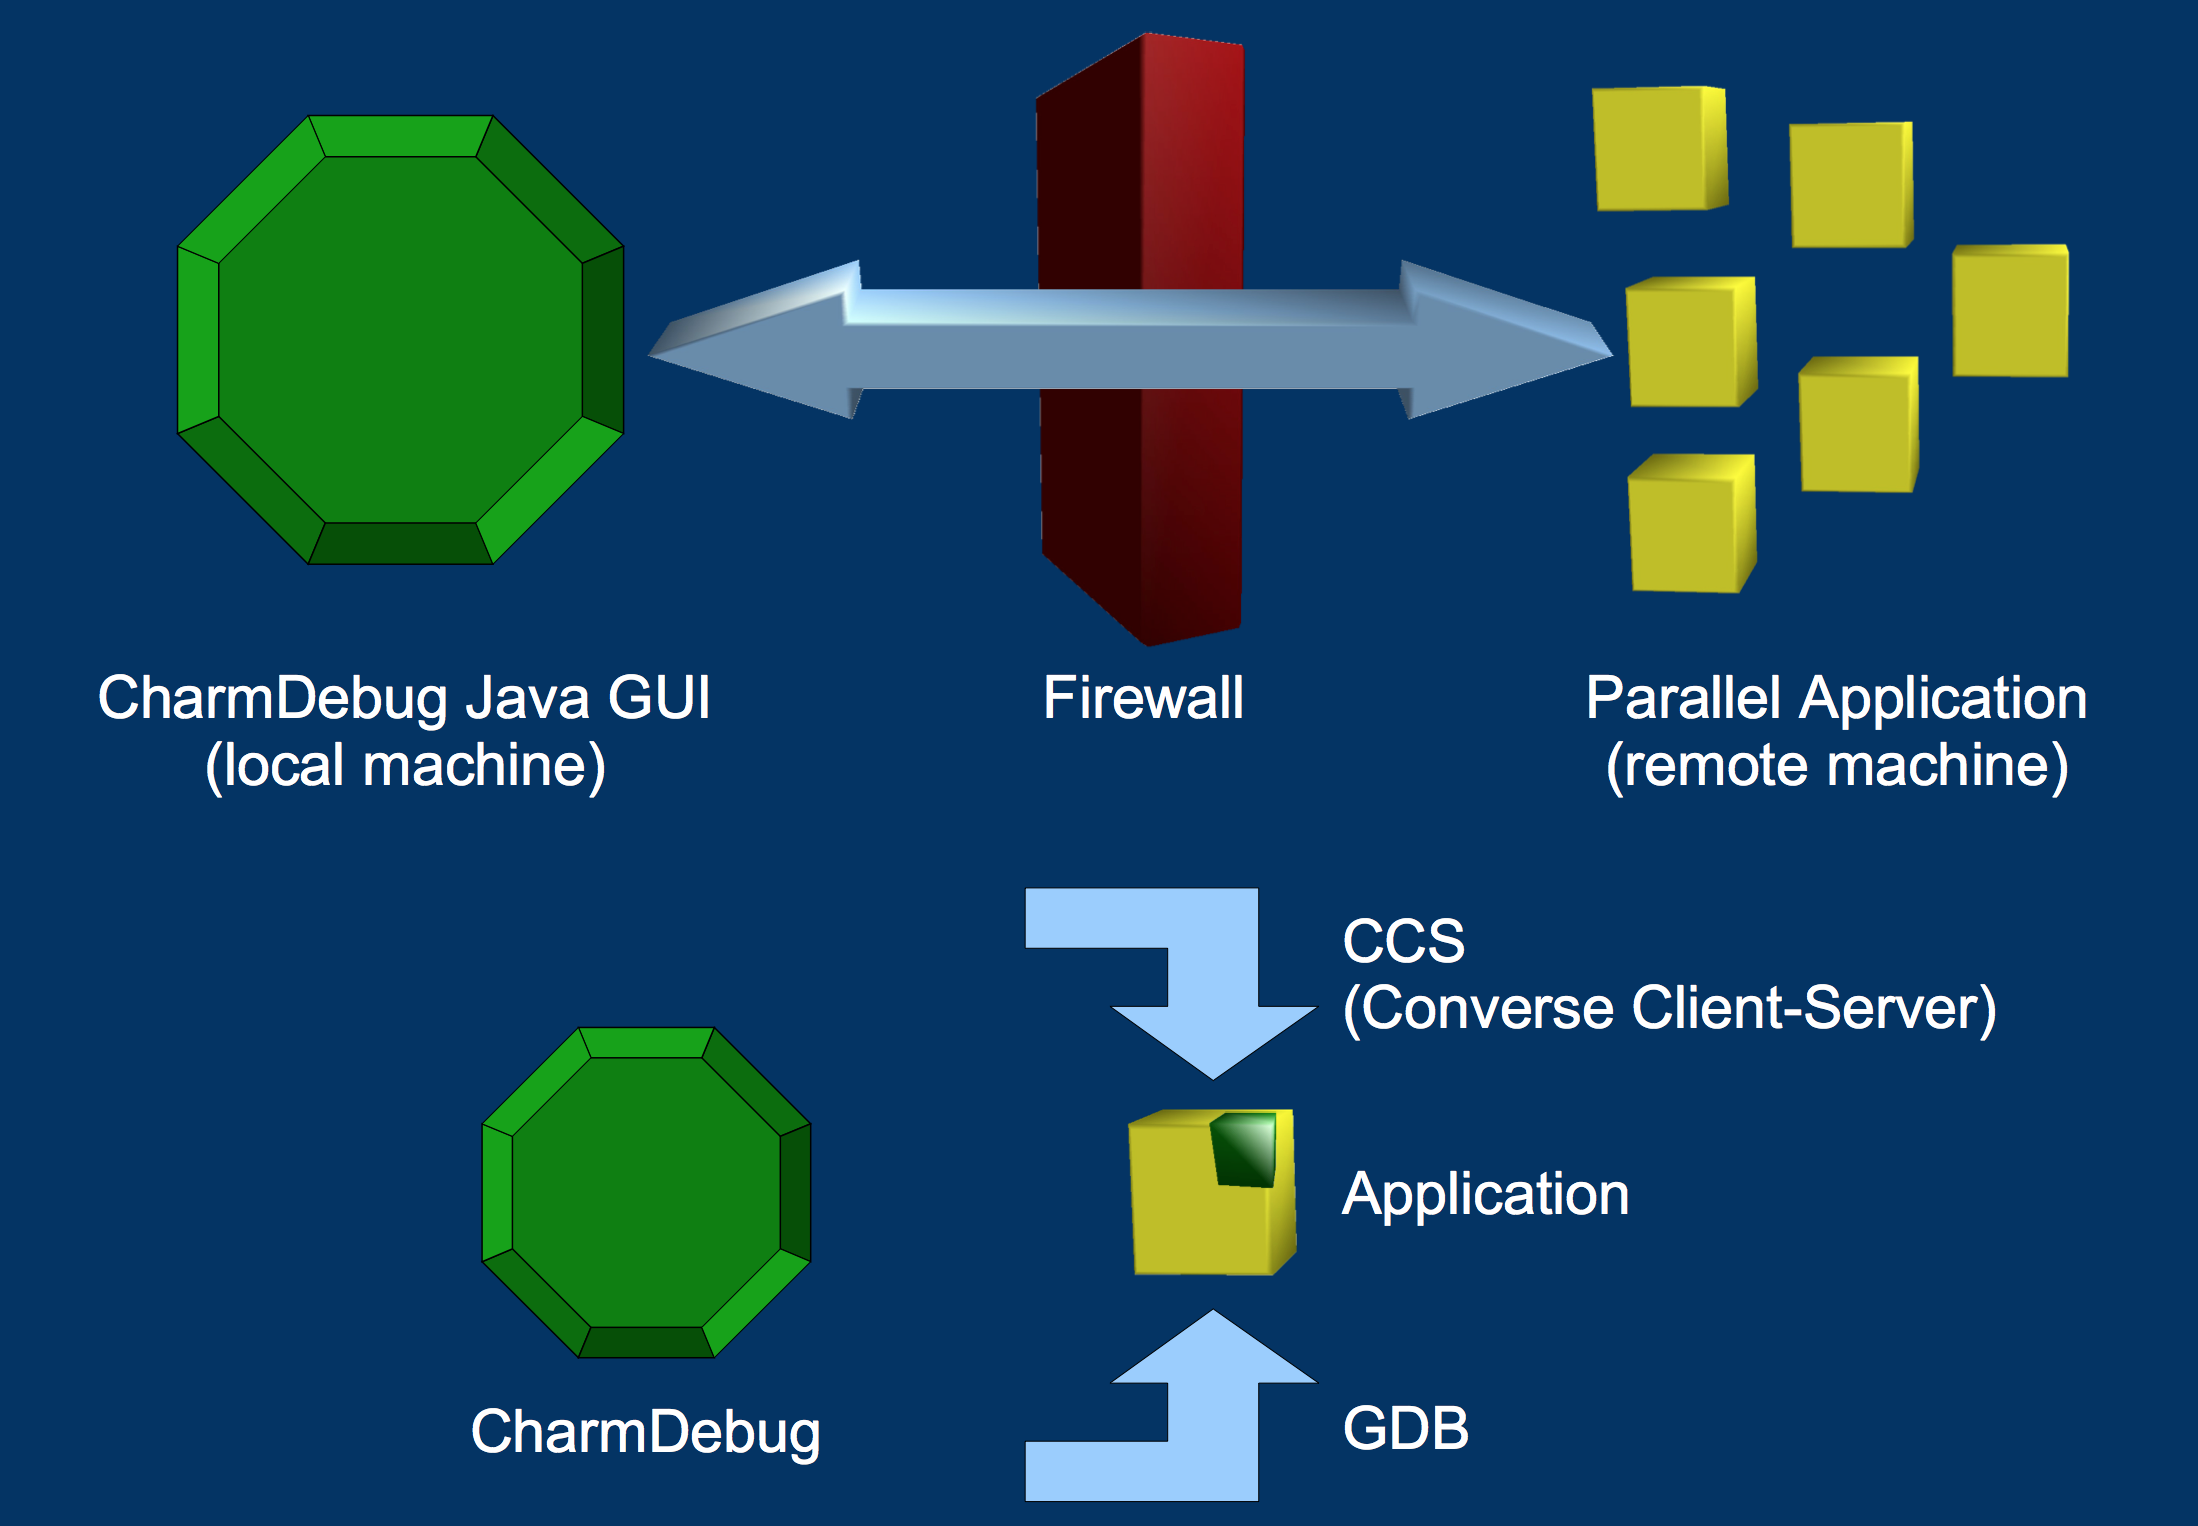
\includegraphics[width=0.9\textwidth]{../figures/overviewDebug.png}\end{center}
\end{frame}

\begin{frame}[fragile]
  \frametitle{Debugging \charm applications using CharmDebug}
  \begin{center}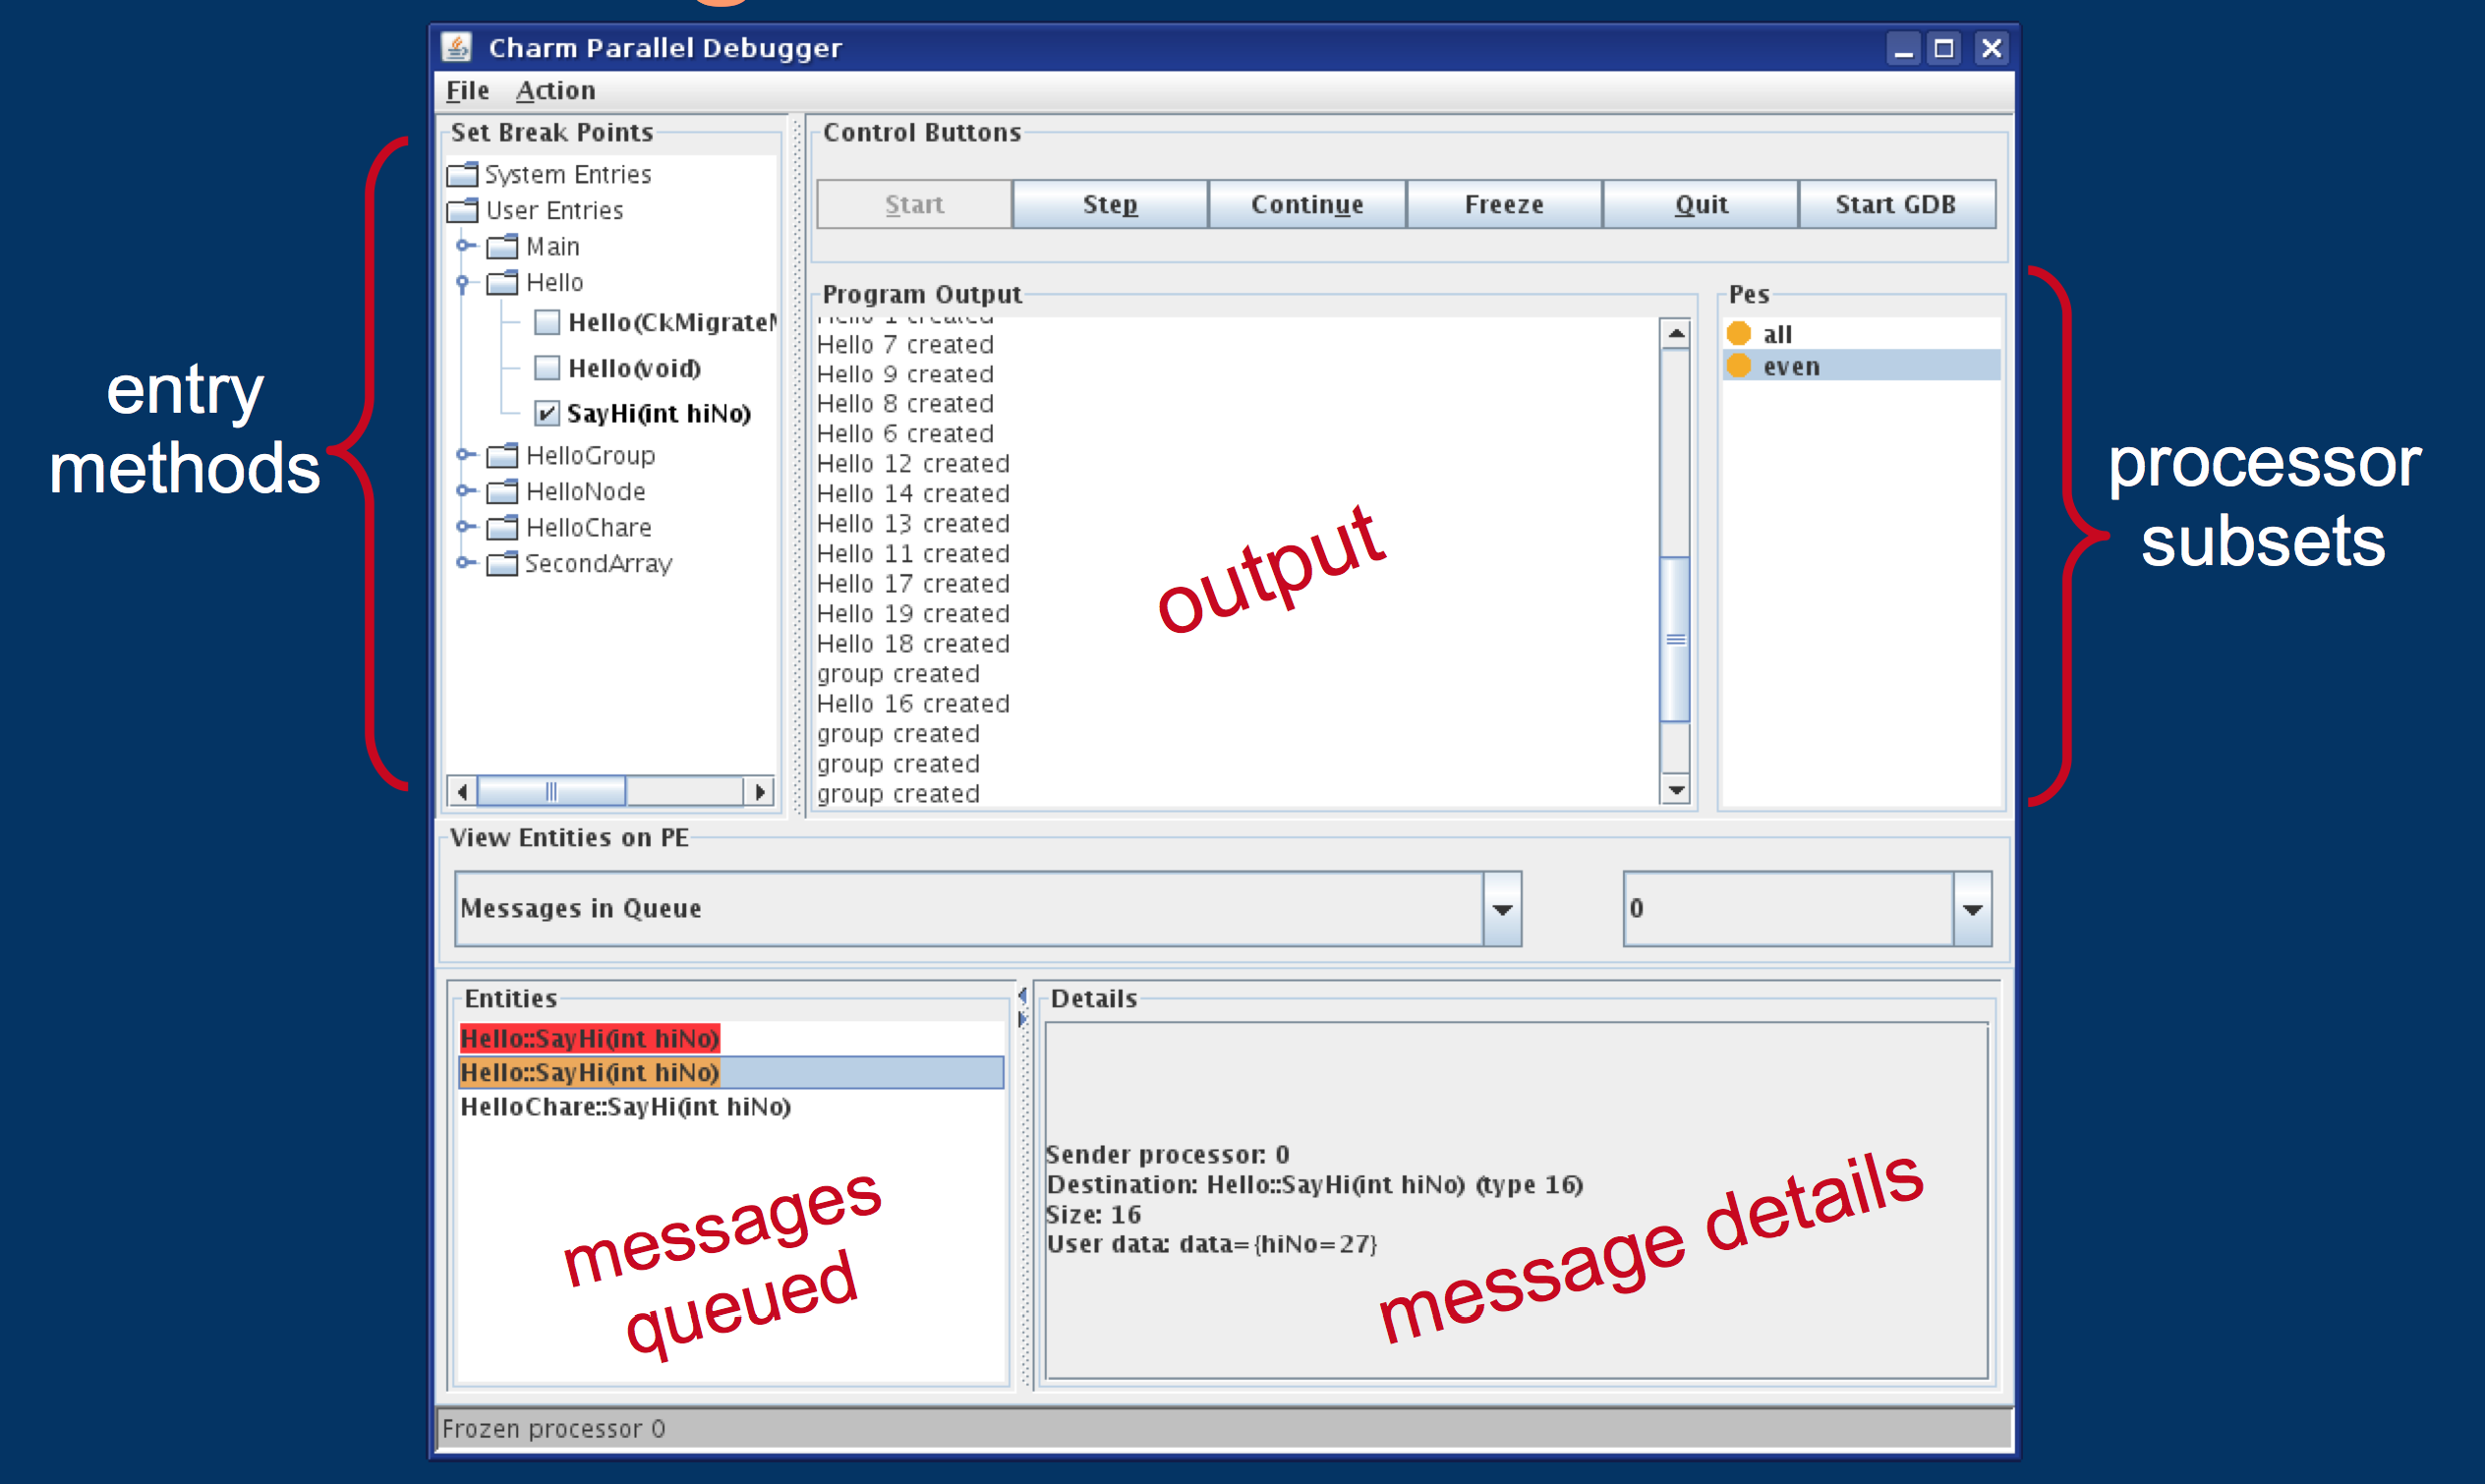
\includegraphics[width=0.9\textwidth]{../figures/debugMainView.png}\end{center}
\end{frame}


\section{Recap}
\begin{frame}
\frametitle{Questions?}
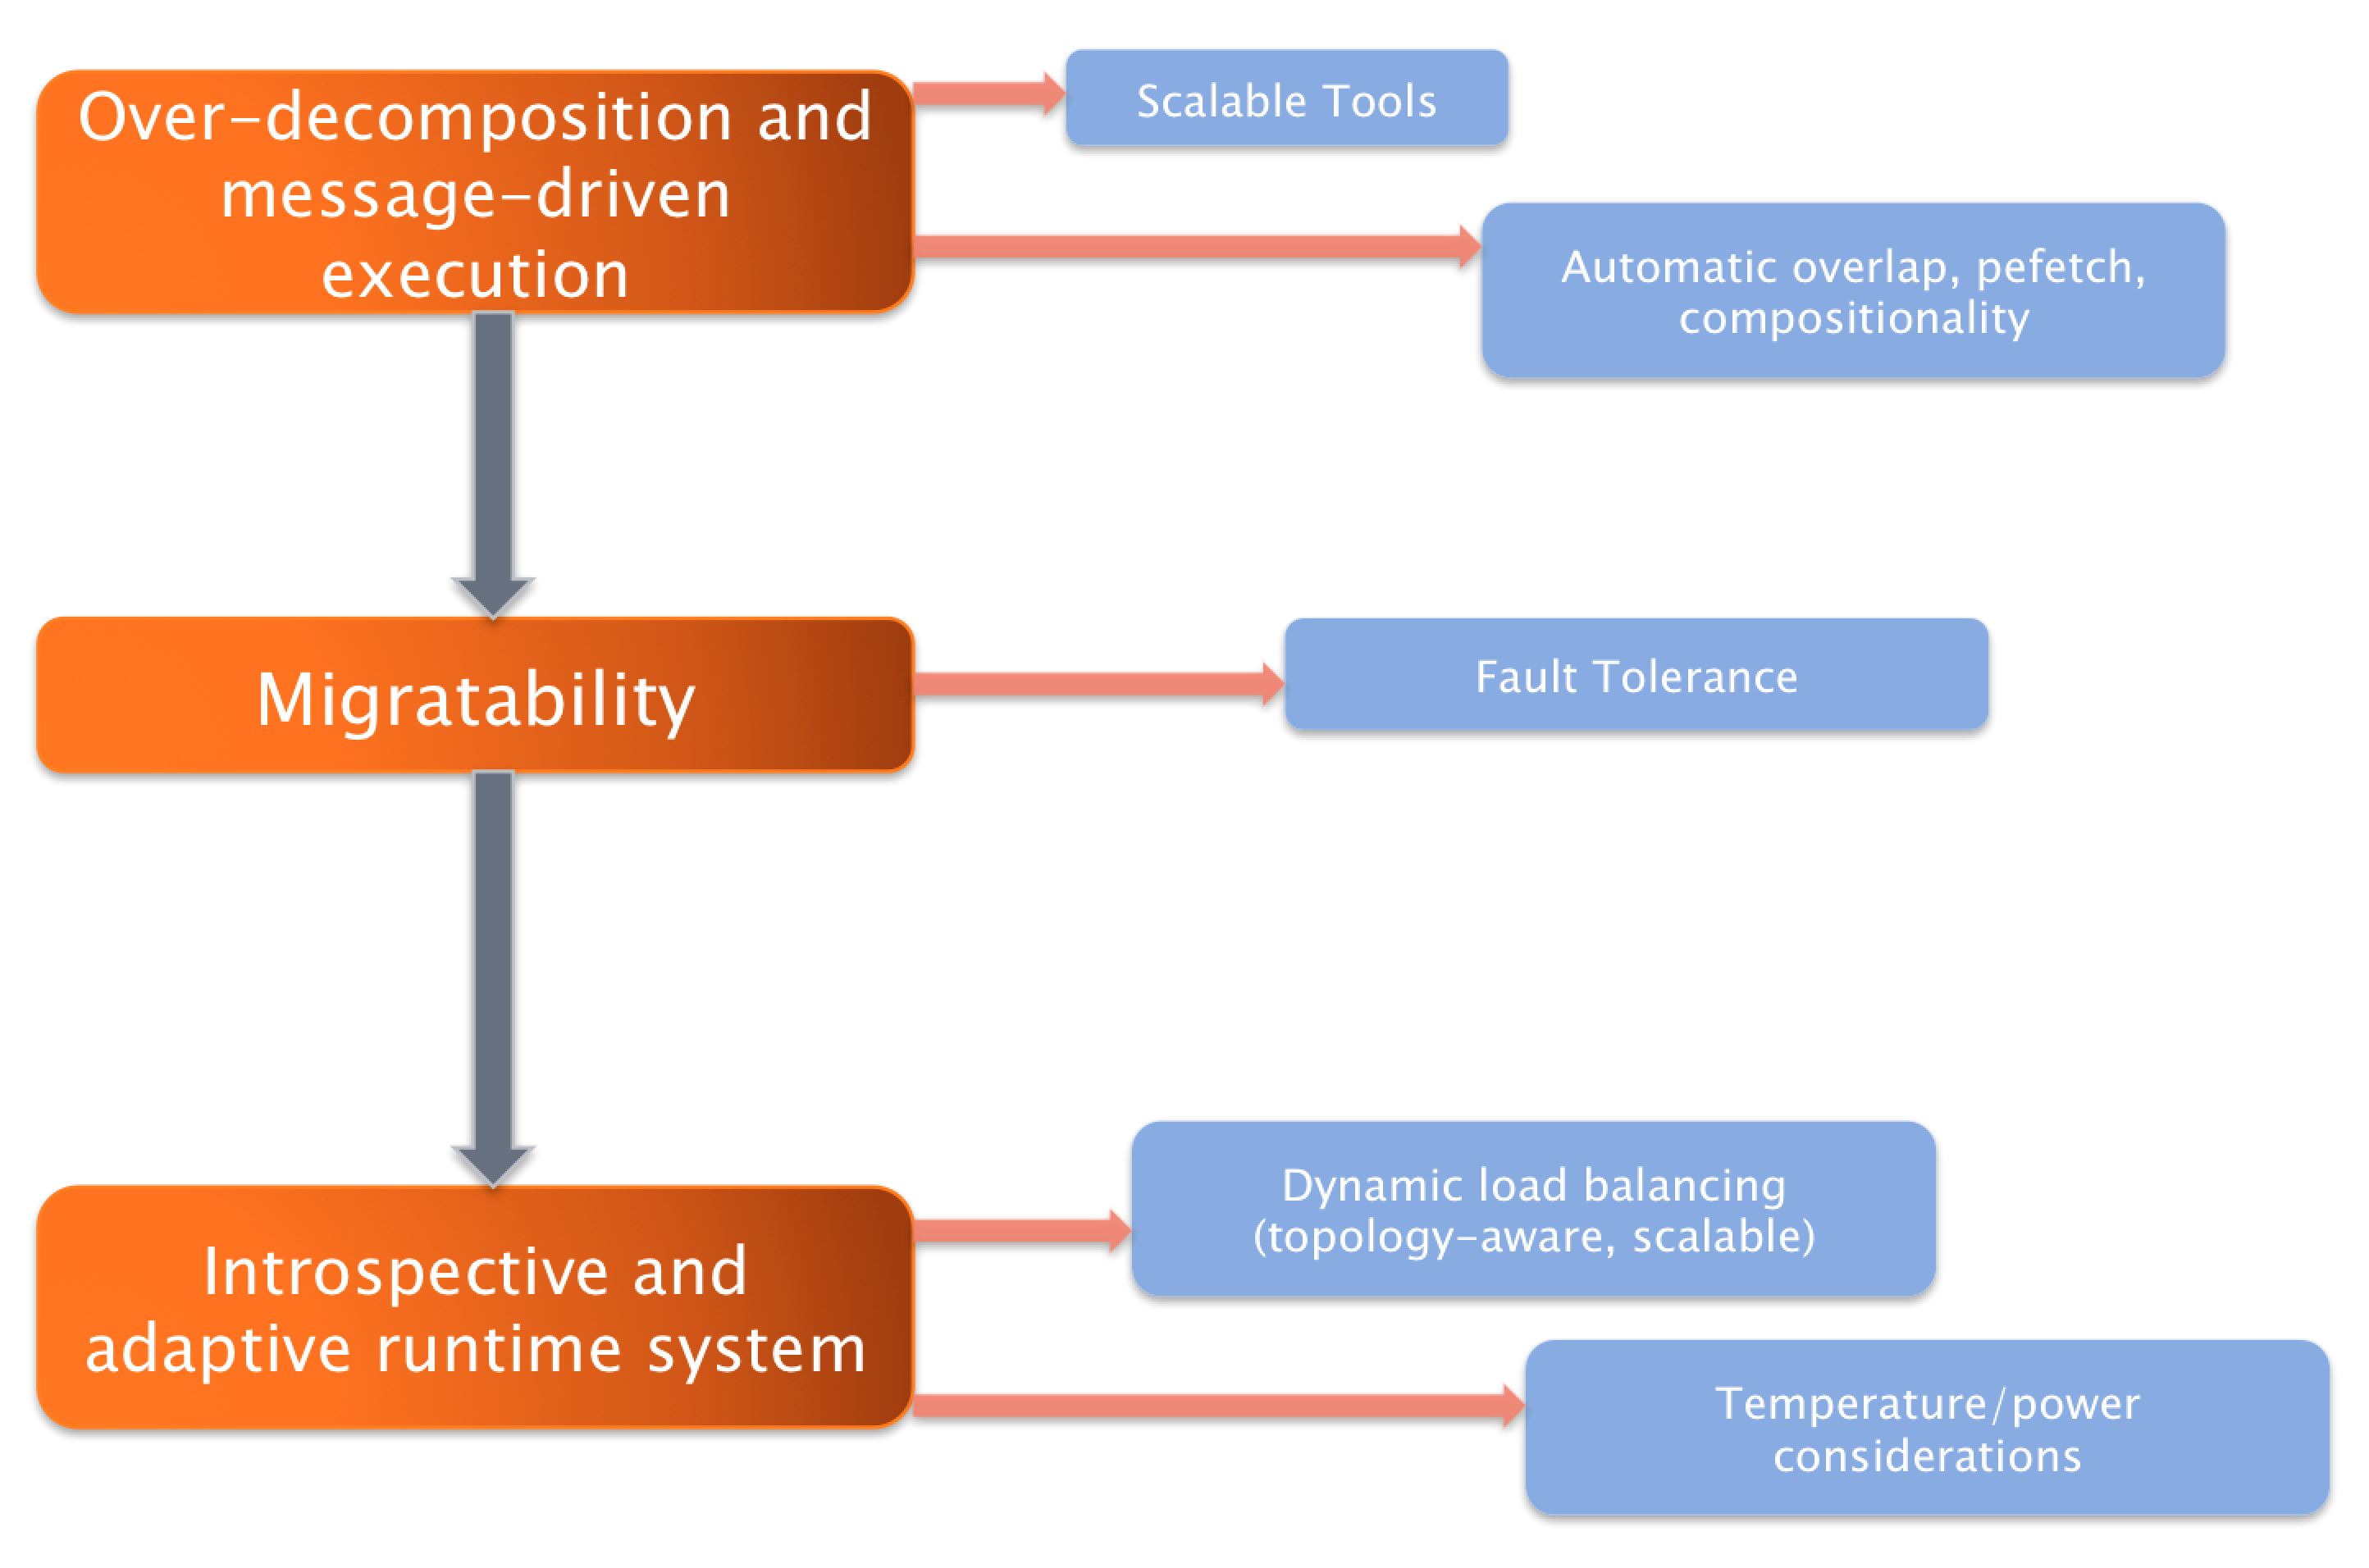
\includegraphics[width=\textwidth]{../figures/charmOutline.png}
\end{frame}


\end{document}

